\documentclass[11pt,a4paper]{article}
% Self-contained: all illustrations are editable TikZ.
% Compile twice with: pdflatex quantum_geometry_visual_guide.tex
\usepackage[T1]{fontenc}
\usepackage[utf8]{inputenc}
\usepackage{lmodern,microtype}
\usepackage[margin=18mm,top=18mm,bottom=19mm,headheight=14pt]{geometry}
\usepackage{amsmath,amssymb,mathtools,bm}
\usepackage{tikz}
\usetikzlibrary{arrows.meta,positioning,calc,decorations.pathreplacing,patterns,fit,shapes.geometric}
\usepackage[most]{tcolorbox}
\usepackage{booktabs,tabularx,array,enumitem,adjustbox,multicol}
\usepackage{fancyhdr,lastpage,hyperref}
\definecolor{KnownBlue}{HTML}{1C5F99}
\definecolor{ProposalGreen}{HTML}{147A54}
\definecolor{CautionAmber}{HTML}{9B6200}
\definecolor{Slate}{HTML}{445267}
\definecolor{Ink}{HTML}{1B2432}
\definecolor{PaleBlue}{HTML}{EDF4FA}
\definecolor{PaleGreen}{HTML}{EDF7F1}
\definecolor{PaleAmber}{HTML}{FFF6E6}
\definecolor{PaleGray}{HTML}{F2F4F7}
\hypersetup{colorlinks=true,linkcolor=KnownBlue,urlcolor=KnownBlue,
pdftitle={Quantum geometry: a visual bridge from undergraduate physics},
pdfauthor={Illustrated study guide},pdfsubject={Bloch states, projectors, geometry, and the three Huang papers}}
\color{Ink}
\pagestyle{fancy}
\fancyhf{}
\fancyhead[L]{\sffamily\footnotesize QUANTUM GEOMETRY / PHYSICS FIRST}
\fancyhead[R]{\sffamily\footnotesize Visual study guide}
\fancyfoot[L]{\sffamily\scriptsize Blue: established \quad Green: proposed extension}
\fancyfoot[R]{\sffamily\scriptsize \thepage/\pageref{LastPage}}
\renewcommand{\headrulewidth}{0.3pt}
\setlength{\parindent}{0pt}
\setlength{\parskip}{5.5pt}
\setlength{\emergencystretch}{2em}
\setlist[itemize]{leftmargin=1.5em,itemsep=3pt,topsep=3pt}
\setlist[enumerate]{leftmargin=1.8em,itemsep=3pt,topsep=3pt}
\newcommand{\ket}[1]{|#1\rangle}
\newcommand{\bra}[1]{\langle#1|}
\newcommand{\Tr}{\operatorname{tr}}
\newcommand{\Ree}{\operatorname{Re}}
\newcommand{\Imm}{\operatorname{Im}}
\newcommand{\Gr}{\operatorname{Gr}}
\newcommand{\Herm}{\operatorname{Herm}}
\newcommand{\CP}{\mathbb{CP}}
\newcommand{\BZ}{T^2}
\newcommand{\dd}{\mathrm d}
\newcommand{\ii}{\mathrm i}
\newcommand{\srctext}[2]{\textcolor{KnownBlue}{\scriptsize\sffamily\hyperlink{ref:#1}{[#1]} #2}}
\newcommand{\src}[2]{\ifmmode\text{\srctext{#1}{#2}}\else\srctext{#1}{#2}\fi}
\newcommand{\esrctext}[1]{\textcolor{ProposalGreen}{\scriptsize\sffamily [E] #1}}
\newcommand{\esrc}[1]{\ifmmode\text{\esrctext{#1}}\else\esrctext{#1}\fi}
\newcommand{\calctext}{\textcolor{Slate}{\scriptsize\sffamily [Calc] standard-mathematics teaching derivation}}
\newcommand{\calc}{\ifmmode\text{\calctext}\else\calctext\fi}
\newcommand{\guidepage}[2]{\clearpage{\sffamily\bfseries\LARGE #1\par}\vspace{3pt}{\sffamily\color{Slate}#2\par}\medskip}
\newcommand{\smallhead}[1]{\par\medskip{\sffamily\bfseries\large #1\par}\vspace{2pt}}
\newtcolorbox{knownbox}[1][]{colback=PaleBlue,colframe=KnownBlue,boxrule=.6pt,arc=2mm,left=3mm,right=3mm,top=2mm,bottom=2mm,before skip=6pt,after skip=6pt,#1}
\newtcolorbox{extensionbox}[1][]{colback=PaleGreen,colframe=ProposalGreen,boxrule=.7pt,arc=2mm,left=3mm,right=3mm,top=2mm,bottom=2mm,before skip=6pt,after skip=6pt,#1}
\newtcolorbox{cautionbox}[1][]{colback=PaleAmber,colframe=CautionAmber,boxrule=.6pt,arc=2mm,left=3mm,right=3mm,top=2mm,bottom=2mm,before skip=6pt,after skip=6pt,#1}
\newtcolorbox{plainbox}[1][]{colback=PaleGray,colframe=Slate!45,boxrule=.5pt,arc=2mm,left=3mm,right=3mm,top=2mm,bottom=2mm,before skip=6pt,after skip=6pt,#1}
\tikzset{
 >={Latex[length=2.2mm]},
 flow/.style={->,line width=.8pt,draw=KnownBlue},
 eflow/.style={->,line width=.9pt,draw=ProposalGreen},
 neutral/.style={draw=Slate,line width=.7pt},
 known/.style={draw=KnownBlue,fill=PaleBlue,rounded corners=2mm,align=center,inner sep=7pt},
 proposed/.style={draw=ProposalGreen,fill=PaleGreen,rounded corners=2mm,align=center,inner sep=7pt},
 caution/.style={draw=CautionAmber,fill=PaleAmber,rounded corners=2mm,align=center,inner sep=7pt},
 basic/.style={draw=Slate!55,fill=PaleGray,rounded corners=2mm,align=center,inner sep=7pt},
 lab/.style={font=\sffamily\scriptsize,align=center},
 every picture/.style={font=\sffamily\small}
}
\begin{document}

% PAGE 1: ORIENTATION
{\sffamily\color{KnownBlue}\bfseries\large AN ILLUSTRATED READING COMPANION\par}
\vspace{4mm}
{\sffamily\bfseries\fontsize{28}{32}\selectfont
From Bloch states\\to curved state spaces\par}
\vspace{3mm}
{\large A physics-first dictionary, relation map, and TikZ story of three papers\par}
\vspace{3mm}
You already know the useful starting objects: a Hamiltonian, its eigenvectors,
inner products, and projectors. Differential geometry organizes how those
objects change as momentum changes. This guide builds that connection before
using the advanced terminology.
\begin{center}
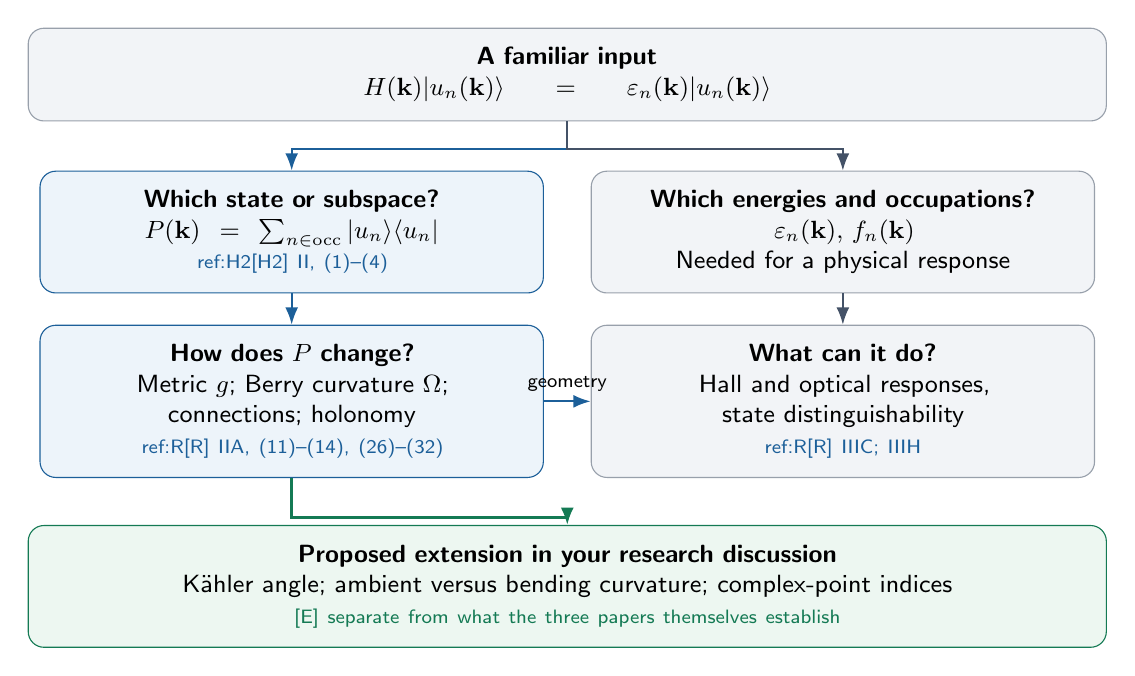
\begin{tikzpicture}
\node[basic,text width=13.2cm] (h) at (0,0)
{\textbf{A familiar input}\\
$H(\mathbf k)\ket{u_n(\mathbf k)}=\varepsilon_n(\mathbf k)\ket{u_n(\mathbf k)}$};
\node[known,text width=5.9cm] (p) at (-3.5,-2.0)
{\textbf{Which state or subspace?}\\
$P(\mathbf k)=\sum_{n\in\mathrm{occ}}\ket{u_n}\bra{u_n}$\\
\src{H2}{II, (1)--(4)}};
\node[basic,text width=5.9cm] (en) at (3.5,-2.0)
{\textbf{Which energies and occupations?}\\
$\varepsilon_n(\mathbf k),\,f_n(\mathbf k)$\\
Needed for a physical response};
\node[known,text width=5.9cm] (geo) at (-3.5,-4.15)
{\textbf{How does $P$ change?}\\
Metric $g$; Berry curvature $\Omega$;\\
connections; holonomy\\
\src{R}{IIA, (11)--(14), (26)--(32)}};
\node[basic,text width=5.9cm] (phys) at (3.5,-4.15)
{\textbf{What can it do?}\\
Hall and optical responses,\\
state distinguishability\\
\src{R}{IIIC; IIIH}};
\draw[flow] (h.south) -- ++(0,-.35) -| (p.north);
\draw[neutral,->] (h.south) -- ++(0,-.35) -| (en.north);
\draw[flow] (p) -- (geo);
\draw[neutral,->] (en) -- (phys);
\draw[flow] (geo) -- node[above,lab]{geometry} (phys);
\node[proposed,text width=13.2cm] (ext) at (0,-6.5)
{\textbf{Proposed extension in your research discussion}\\
K\"ahler angle; ambient versus bending curvature; complex-point indices\\
\esrc{separate from what the three papers themselves establish}};
\draw[eflow] (geo.south) -- ++(0,-.5) -| (ext.north);
\end{tikzpicture}
\end{center}
\begin{tabularx}{\linewidth}{@{}>{\raggedright\arraybackslash}p{3.0cm}X@{}}
\textcolor{KnownBlue}{\textbf{Blue / [H], [R]}} &
Established material used or reported in the cited papers. Blue does not mean
that those authors originally invented the concept.\\[3pt]
\textcolor{ProposalGreen}{\textbf{Green / [E]}} &
The proposed multiband application supplied in this conversation.
Its classical ingredients are cited separately; originality is not certified.\\[3pt]
\textcolor{Slate}{\textbf{Gray / [Calc]}} &
Background or a teaching illustration of standard mathematics.\\[3pt]
\textcolor{CautionAmber}{\textbf{Amber / conditions}} &
Assumptions, distinctions, and questions that remain open.
\end{tabularx}
\smallskip
\textbf{Reading route.} Pages 2--8 build the language; pages 9--10 tell the
three-paper story; pages 11--15 unpack the extension; the final pages connect
to observables, collect conventions, and give a study route.

% PAGE 2: STATE / RAY
\guidepage{1. What is a point in state space?}{Start with a two-component eigenvector, before introducing a manifold.}
A point in momentum space is a value of $\mathbf k$. A point in pure-state
space is a physical state at that value. These are different kinds of points.
For two orbitals,
\[
\ket{u(\mathbf k)}=a(\mathbf k)\ket{\alpha}+b(\mathbf k)\ket{\beta},
\qquad |a|^2+|b|^2=1.
\]
Changing the \emph{relative} amplitudes or phase can change the state. Multiplying
both amplitudes by the same phase cannot change any expectation value.
\src{R}{IIA, pp.\ 4--6}
\begin{center}
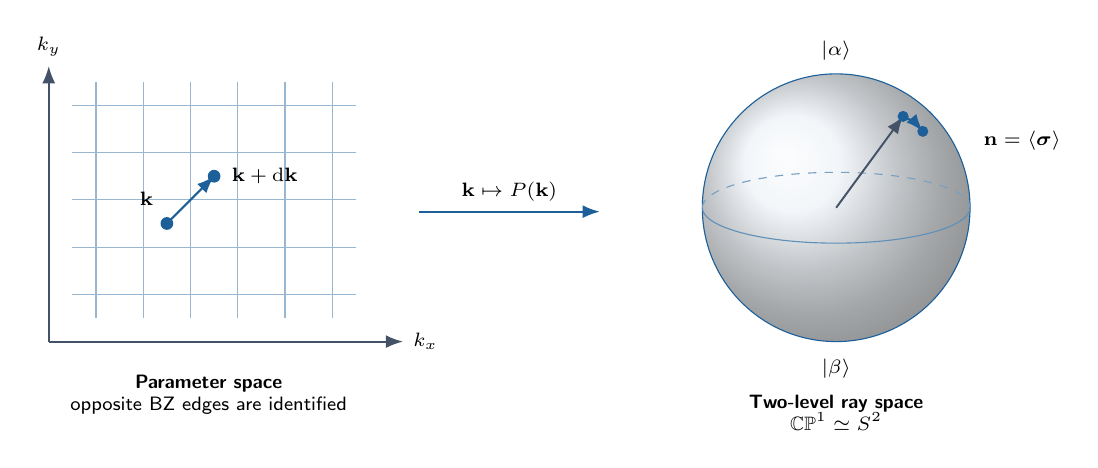
\begin{tikzpicture}
\draw[neutral,->] (0,0)--(4.5,0) node[right,lab]{$k_x$};
\draw[neutral,->] (0,0)--(0,3.5) node[above,lab]{$k_y$};
\draw[KnownBlue!45] (.3,.3) grid[step=.6] (3.9,3.3);
\fill[KnownBlue] (1.5,1.5) circle(2.3pt);
\fill[KnownBlue] (2.1,2.1) circle(2.3pt);
\draw[flow] (1.5,1.5)--(2.1,2.1);
\node[lab,anchor=north west] at (.15,-.3){\textbf{Parameter space}\\opposite BZ edges are identified};
\node[lab,anchor=south east] at (1.45,1.6){$\mathbf k$};
\node[lab,anchor=west] at (2.2,2.1){$\mathbf k+\dd\mathbf k$};
\draw[flow] (4.7,1.65)--(7.0,1.65) node[midway,above,lab]{$\mathbf k\mapsto P(\mathbf k)$};
\begin{scope}[shift={(10.0,1.7)}]
\shade[ball color=KnownBlue!12,opacity=.65] (0,0) circle(1.7);
\draw[KnownBlue] (0,0) circle(1.7);
\draw[KnownBlue!60,dashed] (-1.7,0) arc(180:0:1.7 and .45);
\draw[KnownBlue!70] (-1.7,0) arc(180:360:1.7 and .45);
\draw[neutral,->] (0,0)--(.85,1.16);
\fill[KnownBlue] (.85,1.16) circle(2pt);
\fill[KnownBlue] (1.1,.97) circle(2pt);
\draw[flow] (.85,1.16) to[bend left=12] (1.1,.97);
\node[lab,anchor=south] at (0,1.75){$\ket{\alpha}$};
\node[lab,anchor=north] at (0,-1.8){$\ket{\beta}$};
\node[lab,anchor=west] at (1.75,.85){$\mathbf n=\langle\boldsymbol\sigma\rangle$};
\end{scope}
\node[lab] at (10,-.9){\textbf{Two-level ray space}\\$\CP^1\simeq S^2$};
\end{tikzpicture}
\end{center}
\begin{knownbox}
\textbf{Ray.} The equivalence class of all nonzero multiples of $\ket u$.
Normalized representatives differ by a phase:
\[
\ket u\sim e^{\ii\chi}\ket u,\qquad
P=\ket u\bra u=P^2=P^\dagger .
\]
\textbf{Projective space $\CP^{N-1}$.} The set of all complex rays in
$\mathbb C^N$. A projector is a matrix coordinate for a point in that set.
\hfill\src{H1}{II}\quad\src{R}{IIA, (11), (38)--(43)}
\end{knownbox}
\textbf{Why a manifold?} Near a typical point, a state can be specified by a
small set of smoothly varying real numbers. A sphere needs two local coordinates;
an $N$-component normalized state modulo phase needs $2N-2$ real coordinates.
Different coordinate patches may be needed to cover the whole space.
\textbf{The viewpoint.} Band theory contains both an energy landscape
$\varepsilon_n(\mathbf k)$ and a map of states $P_n(\mathbf k)$.
The Bloch sphere visualizes the second object. It is not an electron
trajectory in real space, a Fermi surface, or an energy surface.
\begin{cautionbox}
The zero-metric atomic limit in the review's Fig.\ 1 has a
momentum-independent state. A topologically trivial band with $C=0$ can still
have nonzero local metric and Berry curvature.
\src{R}{Fig.\ 1, p.\ 2; IIA}
\end{cautionbox}

% PAGE 3: SUBSPACE / BUNDLE
\guidepage{2. Several occupied bands form a moving plane}{Grassmannian, frame, gauge, and bundle in linear-algebra language.}
Suppose a gap separates $r$ occupied bands from $N-r$ unoccupied bands.
Collect an orthonormal occupied frame in an $N\times r$ matrix $\Psi$:
\[
\Psi^\dagger\Psi=I_r,\qquad P=\Psi\Psi^\dagger,\qquad
\Psi\mapsto\Psi U,\quad U\in U(r).
\]
The last change rotates the chosen occupied basis while preserving $P$.
It preserves subspace geometry even when individual energies differ; it
need not preserve the diagonal form of the Hamiltonian.
\src{H2}{II, (1)--(4)}
\begin{center}
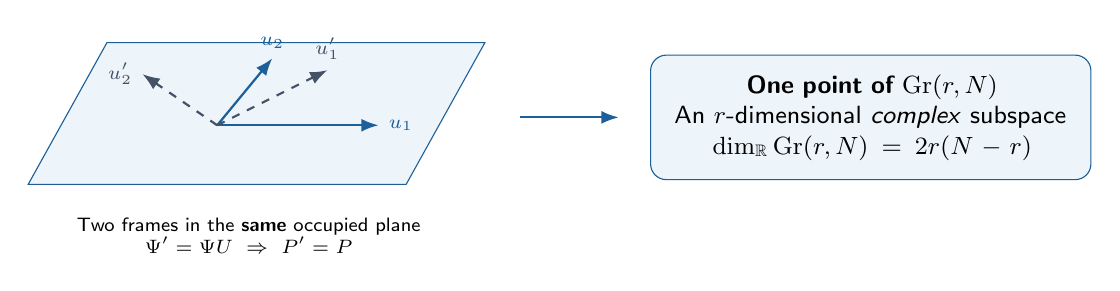
\begin{tikzpicture}
\begin{scope}
\fill[PaleBlue] (0,0)--(4.8,0)--(5.8,1.8)--(1,1.8)--cycle;
\draw[KnownBlue] (0,0)--(4.8,0)--(5.8,1.8)--(1,1.8)--cycle;
\coordinate (o) at (2.4,.75);
\draw[->,KnownBlue,thick] (o)--(4.45,.75) node[right,lab]{$u_1$};
\draw[->,KnownBlue,thick] (o)--(3.1,1.6) node[above,lab]{$u_2$};
\draw[->,Slate,dashed,thick] (o)--(3.8,1.45) node[above,lab]{$u'_1$};
\draw[->,Slate,dashed,thick] (o)--(1.45,1.4) node[left,lab]{$u'_2$};
\node[lab] at (2.8,-.65){Two frames in the \textbf{same} occupied plane\\$\Psi'=\Psi U\ \Rightarrow\ P'=P$};
\end{scope}
\draw[flow] (6.25,.85)--(7.5,.85);
\node[known,text width=5.1cm] at (10.7,.85)
{\textbf{One point of $\Gr(r,N)$}\\
An $r$-dimensional \emph{complex} subspace\\
$\dim_{\mathbb R}\Gr(r,N)=2r(N-r)$};
\end{tikzpicture}
\end{center}
\textbf{Grassmannian.} The collection of all such occupied subspaces:
\[
\Gr(r,N)=\frac{U(N)}{U(r)\times U(N-r)}.
\]
The denominator removes rotations within the occupied and unoccupied sectors.
Only rotations that mix the sectors change the point $P$.
\src{H1}{II}\quad\src{H2}{II}
\begin{center}
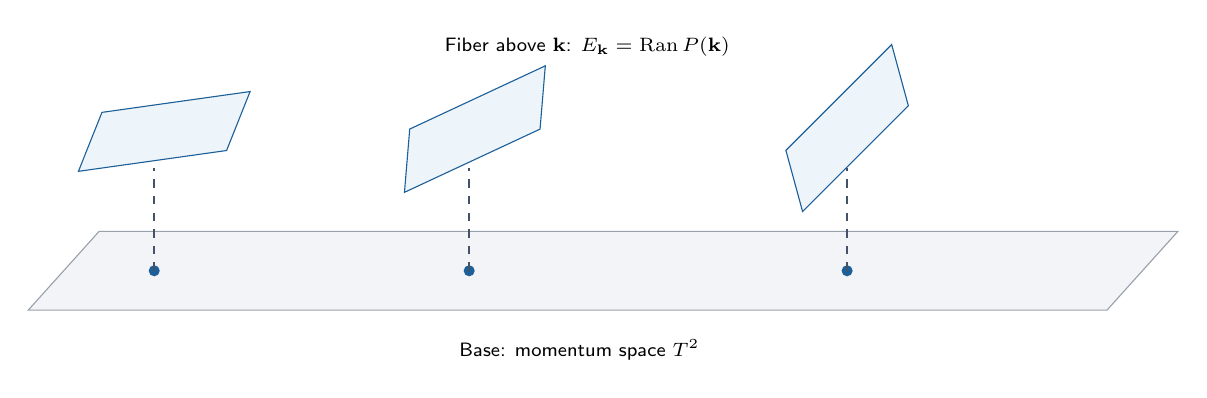
\begin{tikzpicture}
\fill[PaleGray] (0,0)--(13.7,0)--(14.6,1)--(.9,1)--cycle;
\draw[Slate!55] (0,0)--(13.7,0)--(14.6,1)--(.9,1)--cycle;
\foreach \x/\ang in {1.6/8,5.6/25,10.4/45}{
 \fill[KnownBlue] (\x,.5) circle(2pt);
 \draw[neutral,dashed] (\x,.5)--(\x,1.8);
 \begin{scope}[shift={(\x,2.1)},rotate=\ang]
 \fill[PaleBlue] (-1,-.2)--(.9,-.2)--(1.3,.5)--(-.6,.5)--cycle;
 \draw[KnownBlue] (-1,-.2)--(.9,-.2)--(1.3,.5)--(-.6,.5)--cycle;
 \end{scope}
}
\node[lab,anchor=north] at (7,-.25){Base: momentum space $T^2$};
\node[lab,anchor=south] at (7.1,3.1){Fiber above $\mathbf k$: $E_{\mathbf k}=\operatorname{Ran}P(\mathbf k)$};
\end{tikzpicture}
\end{center}
\textbf{Vector bundle $E\to T^2$.} Keep a copy of the occupied vector space
attached to each momentum. The fibers vary smoothly while the separating
gap stays open. A \textbf{local frame} is a smooth basis on a patch.
A \textbf{section} chooses one vector in each fiber.
A nonzero Chern number obstructs a globally smooth periodic occupied frame,
while $P$ can remain globally smooth.
\src{H2}{I--II}
\begin{plainbox}
\textbf{Keep four objects separate:}\quad
base $T^2$;\ target $\Gr(r,N)$;\ image $P(T^2)$;\ occupied bundle $E$.
The parameterization is regular at $\mathbf k$ exactly when $\dd P_{\mathbf k}$
has rank two. Each sufficiently small regular source patch describes a smooth
two-dimensional sheet. The complete image may have overlapping sheets or
self-intersections.
The full Grassmannian usually has many more dimensions.
All drawn planes are real sketches of complex vector spaces.
\end{plainbox}

% PAGE 4: DISTANCE / PULLBACK
\guidepage{3. Distance becomes a metric by zooming in}{A finite comparison, its infinitesimal limit, and the meaning of pullback.}
For two rays, define the principal angle
$\vartheta=\arccos|\langle u|v\rangle|$. For two occupied subspaces,
the singular values of $\Psi_1^\dagger\Psi_2$ are $\cos\vartheta_a$.
These angles do not depend on the frames used.
\src{H1}{II, (4)--(5)}
\begin{center}
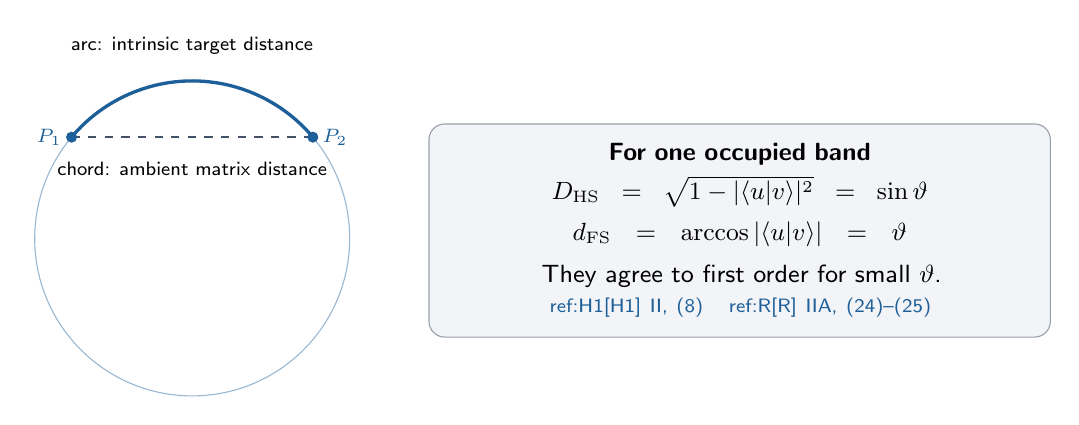
\begin{tikzpicture}
\draw[KnownBlue!45] (0,0) circle(2);
\coordinate (a) at (-1.532,1.286);
\coordinate (b) at (1.532,1.286);
\draw[KnownBlue,very thick] (a) arc(140:40:2);
\draw[Slate,dashed,thick] (a)--(b);
\fill[KnownBlue] (a) circle(2pt) node[left,lab]{$P_1$};
\fill[KnownBlue] (b) circle(2pt) node[right,lab]{$P_2$};
\node[lab] at (0,2.45){arc: intrinsic target distance};
\node[lab] at (0,.88){chord: ambient matrix distance};
\node[basic,text width=7.4cm,anchor=west] at (3.0,.1)
{\textbf{For one occupied band}\\[3pt]
$D_{\rm HS}=\sqrt{1-|\langle u|v\rangle|^2}=\sin\vartheta$\\[4pt]
$d_{\rm FS}=\arccos|\langle u|v\rangle|=\vartheta$\\[4pt]
They agree to first order for small $\vartheta$.\\
\src{H1}{II, (8)}\quad\src{R}{IIA, (24)--(25)}};
\end{tikzpicture}
\end{center}
\begin{knownbox}
\[
D_{\rm HS}^2(P_1,P_2)
=\frac12\Tr(P_1-P_2)^2
=\sum_a\sin^2\vartheta_a.
\qquad\text{\src{H1}{II, (8)}}
\]
For $P_2=P(\mathbf k+\dd\mathbf k)$, expand the projector:
\[
D_{\rm HS}^2=g_{ij}\,\dd k^i\dd k^j+O(|\dd\mathbf k|^3),
\qquad
g_{ij}=\frac12\Tr[(\partial_iP)(\partial_jP)].
\]
\hfill\src{R}{IIA, (13), (17)}\quad\src{H2}{IV.2, (27), rescaled}
\end{knownbox}
\textbf{Metric.} A rule that turns a small displacement into a squared length.
Here the length means a change of occupied subspace.
\begin{center}
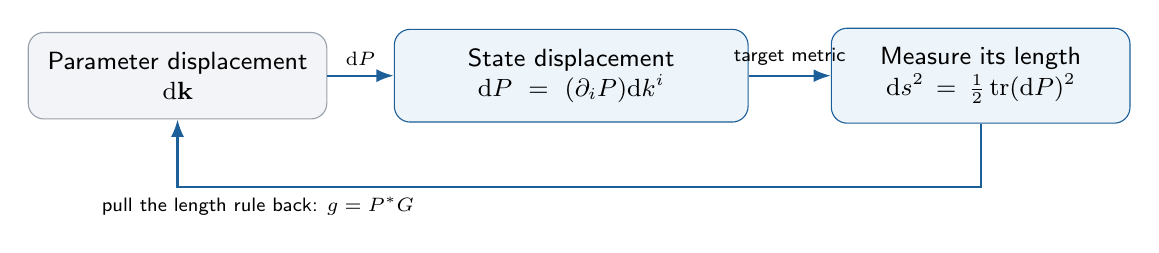
\begin{tikzpicture}
\node[basic,text width=3.3cm] (dk) at (0,0)
{Parameter displacement\\$\dd\mathbf k$};
\node[known,text width=4.0cm] (dp) at (5.0,0)
{State displacement\\$\dd P=(\partial_iP)\dd k^i$};
\node[known,text width=3.3cm] (ds) at (10.2,0)
{Measure its length\\$\dd s^2=\frac12\Tr(\dd P)^2$};
\draw[flow] (dk)--node[above,lab]{$\dd P$}(dp);
\draw[flow] (dp)--node[above,lab]{target metric}(ds);
\draw[flow] (ds.south)--++(0,-.8)-|
 node[pos=.45,below,lab]{pull the length rule back: $g=P^*G$}(dk.south);
\end{tikzpicture}
\end{center}
\textbf{Pullback.} Transfer a measurement rule from the target to the input
coordinates. In the elementary analogy $\mathbf r(x^1,x^2)$,
$g_{ij}=\partial_i\mathbf r\cdot\partial_j\mathbf r$ does exactly this.
Replacing $\mathbf r$ by $P$ gives the quantum version. No inverse map is needed.
\src{MO}{II and Appendix A}
\begin{cautionbox}
A shortest path in the full Grassmannian can leave the physical image $P(T^2)$.
H1's disparity $\frac2\pi\sum_a\vartheta_a$ and the standard geodesic distance
$\sqrt{\sum_a\vartheta_a^2}$ are different finite quantities.
\src{H1}{II, (5)}\quad\src{H2}{IV.3--IV.4, (61)}
\end{cautionbox}

% PAGE 5: QGT
\guidepage{4. The QGT is a Gram matrix of state changes}{This is where perturbation theory becomes geometry.}
For one isolated band, split the derivative into a phase part and a physical
change:
\[
\ket{\partial_i u}
=P\ket{\partial_i u}+Q\ket{\partial_i u},
\qquad Q=I-P,\qquad
\ket{D_i u}:=Q\ket{\partial_i u}.
\]
$P\ket{\partial_i u}$ only changes the representative's phase; the orthogonal
part changes the ray. This is the concrete meaning of a
\textbf{horizontal derivative}.
\src{R}{IIA, (8)--(12), Fig.\ 2}
\begin{center}
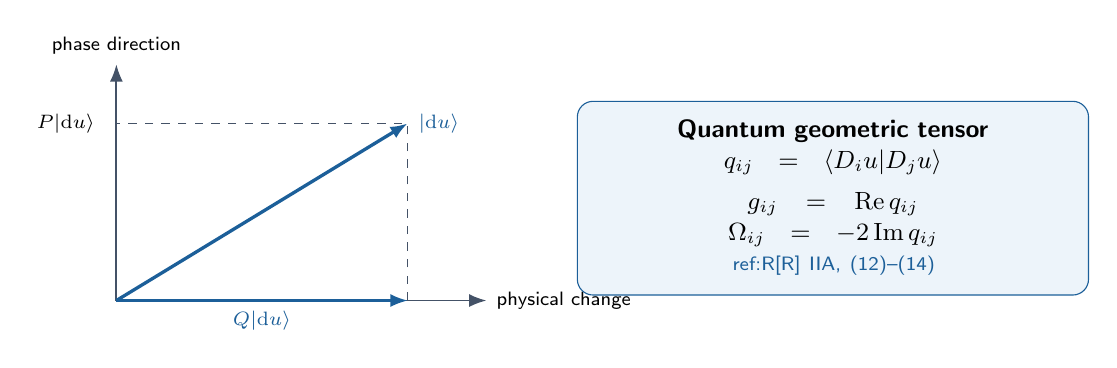
\begin{tikzpicture}
\draw[neutral,->] (0,0)--(0,3.0) node[above,lab]{phase direction};
\draw[neutral,->] (0,0)--(4.7,0) node[right,lab]{physical change};
\draw[KnownBlue,->,very thick] (0,0)--(3.7,2.25)
 node[right,lab]{$\ket{\dd u}$};
\draw[KnownBlue,->,thick] (0,0)--(3.7,0)
 node[midway,below,lab]{$Q\ket{\dd u}$};
\draw[Slate,dashed] (3.7,0)--(3.7,2.25)--(0,2.25);
\node[lab,anchor=east] at (-.15,2.25){$P\ket{\dd u}$};
\node[known,text width=6.0cm] at (9.1,1.3)
{\textbf{Quantum geometric tensor}\\
$q_{ij}=\langle D_i u|D_j u\rangle$\\[4pt]
$g_{ij}=\Ree q_{ij}$\\
$\Omega_{ij}=-2\Imm q_{ij}$\\
\src{R}{IIA, (12)--(14)}};
\end{tikzpicture}
\end{center}
\textbf{Two aspects of the same local data.} The real inner product measures
lengths and angles of state changes. The imaginary part gives the Berry phase
per small oriented loop area:
\[
\dd s^2=g_{ij}\dd k^i\dd k^j,\qquad
\gamma_{\square}=\Omega_{xy}\,\delta k_x\delta k_y+
\text{higher orders}.
\]
\hfill\src{R}{IIA, (4), (7), (9), (14)}
\smallhead{A formula you can recognize from perturbation theory}
Differentiating $H\ket{u_n}=\varepsilon_n\ket{u_n}$ gives, for $m\ne n$,
\[
\langle u_m|\partial_i u_n\rangle
=\frac{\langle u_m|\partial_iH|u_n\rangle}{\varepsilon_n-\varepsilon_m}.
\quad\src{R}{IIA, (36)}
\]
Therefore
\begin{knownbox}
\[
q^{(n)}_{ij}
=\sum_{m\ne n}
\frac{\langle u_n|\partial_iH|u_m\rangle
      \langle u_m|\partial_jH|u_n\rangle}
     {(\varepsilon_n-\varepsilon_m)^2}.
\qquad\text{\src{R}{IIA, (37)}}
\]
\textbf{Physics picture:} momentum changes admix other bands into $\ket{u_n}$.
The metric measures the size of that admixture, and the imaginary
cross-correlation supplies Berry curvature.
\end{knownbox}
In a fixed Bloch basis, $\partial_iH=\hbar v_i$. The same interband
matrix elements also enter response theory. A small gap can enhance geometry
when the numerator is nonzero; a small gap alone does not force an enhancement.

\textbf{For an occupied multiplet,} remove mixing inside the whole occupied
subspace: $B_i=Q(\partial_iP)P$. Then
$q_{ij}=\Tr(B_i^\dagger B_j)$.
The traced QGT does not contain every component of the matrix-valued
non-Abelian curvature.
\src{H2}{IV.1--IV.2, (24)--(30)}

% PAGE 6: WORKED SPINOR
\guidepage{5. Work out one Bloch sphere completely}{One calculation fixes metric, area, curvature, and signs.}
Use a normalized state on a regular sphere-coordinate patch:
\[
\ket{u(\theta,\phi)}
=\begin{pmatrix}\cos(\theta/2)\\e^{\ii\phi}\sin(\theta/2)\end{pmatrix},
\qquad 0<\theta<\pi.
\]
Its Bloch vector is
$\mathbf n=(\sin\theta\cos\phi,\sin\theta\sin\phi,\cos\theta)$, and
$P=(I+\mathbf n\cdot\boldsymbol\sigma)/2$.
\src{R}{IIA, (38)--(45)}
\begin{center}
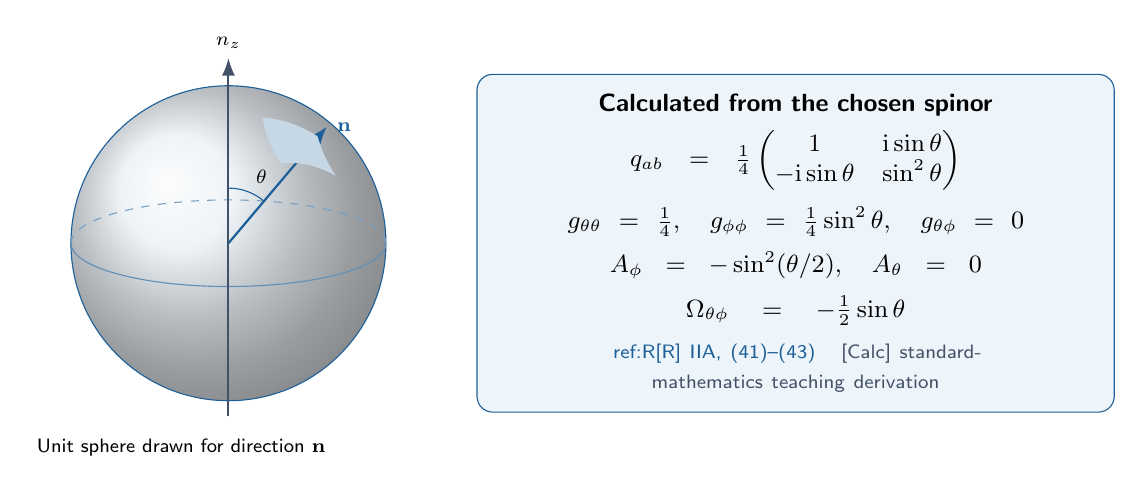
\begin{tikzpicture}
\begin{scope}
\shade[ball color=KnownBlue!14,opacity=.7] (0,0) circle(2);
\draw[KnownBlue] (0,0) circle(2);
\draw[KnownBlue!60,dashed] (-2,0) arc(180:0:2 and .55);
\draw[KnownBlue!70] (-2,0) arc(180:360:2 and .55);
\draw[neutral,->] (0,-2.2)--(0,2.35) node[above,lab]{$n_z$};
\draw[KnownBlue,->,thick] (0,0)--(1.25,1.48) node[right,lab]{$\mathbf n$};
\draw[KnownBlue] (0,.7) arc(90:50:.7);
\node[lab] at (.42,.85){$\theta$};
\fill[KnownBlue!25] (.43,1.6) to[bend left=12] (1.13,1.36)
to[bend right=8] (1.36,.86) to[bend right=15] (.66,1.02)
to[bend left=10] cycle;
\node[lab] at (-.6,-2.6){Unit sphere drawn for direction $\mathbf n$};
\end{scope}
\node[known,text width=7.6cm,anchor=west] at (3.15,0)
{\textbf{Calculated from the chosen spinor}\\[4pt]
$q_{ab}=\frac14
\begin{pmatrix}
1&\ii\sin\theta\\
-\ii\sin\theta&\sin^2\theta
\end{pmatrix}$\\[5pt]
$g_{\theta\theta}=\frac14,\quad g_{\phi\phi}=\frac14\sin^2\theta,
\quad g_{\theta\phi}=0$\\[5pt]
$A_\phi=-\sin^2(\theta/2),\quad A_\theta=0$\\[5pt]
$\Omega_{\theta\phi}=-\frac12\sin\theta$\\[4pt]
\src{R}{IIA, (41)--(43)}\quad\calc};
\end{tikzpicture}
\end{center}
\textbf{Two different uses of $A$.}
$A_a=\ii\langle u|\partial_a u\rangle$ is the Berry connection for the
chosen phase convention. The symbol $\dd A$ below denotes the quantum
area element. The QGT fixes $g$ and $\Omega$, but does not fix a gauge
choice for $A_a$.
\src{R}{IIA, (4), (6)--(14)}
\begin{knownbox}
\[
\dd s^2=\frac14(\dd\theta^2+\sin^2\theta\,\dd\phi^2),\qquad
\dd A=\frac14\sin\theta\,\dd\theta\,\dd\phi,\qquad K_G=4.
\]
The metric is that of a sphere of radius $1/2$.
For this band's orientation,
$\Omega_{\theta\phi}\dd\theta\dd\phi=-2\,\dd A$.
A loop enclosing oriented solid angle $\mathcal S$ on the
\emph{unit} Bloch sphere has Berry phase $-\mathcal S/2$ modulo $2\pi$.
\end{knownbox}
\textbf{An immediate distinction between two curvatures.}
The orthogonal state has the same metric and the opposite Berry curvature:
\[
g_+=g_-,\qquad \Omega_+=-\Omega_-.
\quad\src{R}{IIA, (41)}
\]
Its intrinsic Gaussian curvature is still $4$.
Berry curvature therefore cannot generally be identified with the
Gaussian curvature computed from $g$.

\textbf{Pull this result back to a band.}
For $\theta(\mathbf k)$ and $\phi(\mathbf k)$, the chain rule gives
$g_{ij}=\frac14\partial_i\mathbf n\cdot\partial_j\mathbf n$ and
$\Omega_{ij}=-\frac12\mathbf n\cdot(\partial_i\mathbf n\times\partial_j\mathbf n)$
for $P=(I+\mathbf n\cdot\boldsymbol\sigma)/2$.
On a rank-two patch, $K_G$ remains $4$.
\begin{cautionbox}
\textbf{Coordinate singularity versus rank loss.}
The poles are singularities of $(\theta,\phi)$ coordinates, not of the sphere.
A fold of $\mathbf k\mapsto P(\mathbf k)$ is different: a genuine nonzero
momentum direction produces $\dd P=0$.
Use regular momentum coordinates to test that condition.
\end{cautionbox}

% PAGE 7: CONNECTIONS
\guidepage{6. Connection means a rule for comparison}{Always ask: what object is being transported?}
Vectors at neighboring points may be written in different local frames.
A \textbf{connection} specifies how to compare them.
A \textbf{covariant derivative} corrects an ordinary derivative for the
frame's change. \textbf{Holonomy} is the net transformation after a closed trip.

The \textbf{Euler characteristic} in the right-hand column counts
$\chi=V-E+F$ for a triangulated surface. For a closed orientable surface with
$h$ handles, $\chi=2-2h$: a sphere has $2$; a torus has $0$.
It concerns the surface itself, whereas $C$ below concerns its occupied bundle.
\calc
\begin{center}
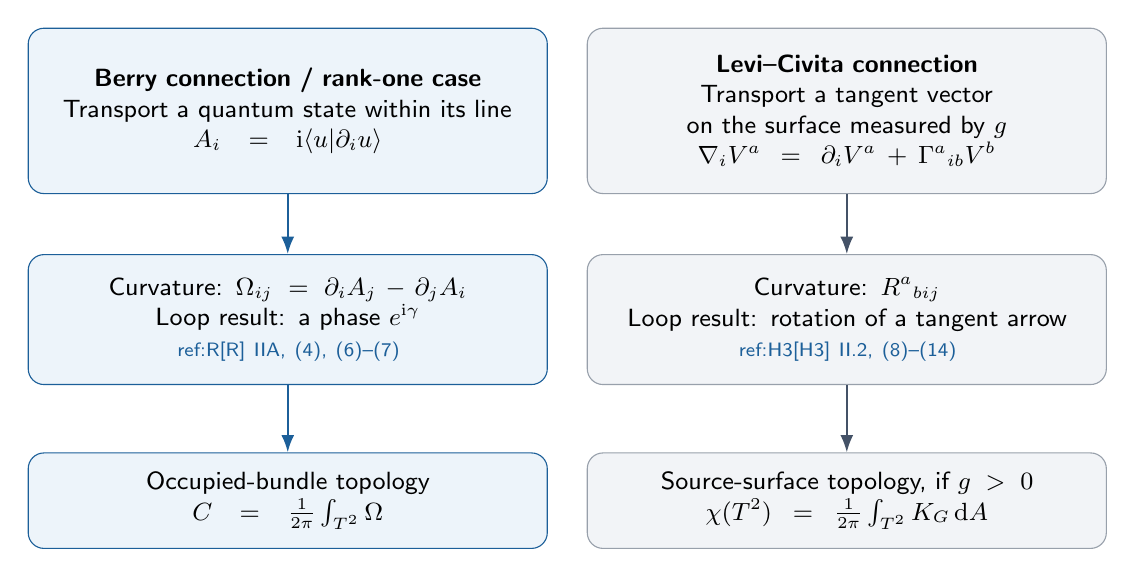
\begin{tikzpicture}
\node[known,text width=6.1cm,minimum height=2.1cm] (b1) at (-3.55,0)
{\textbf{Berry connection / rank-one case}\\
Transport a quantum state within its line\\
$A_i=\ii\langle u|\partial_i u\rangle$};
\node[basic,text width=6.1cm,minimum height=2.1cm] (b2) at (3.55,0)
{\textbf{Levi--Civita connection}\\
Transport a tangent vector on the surface measured by $g$\\
$\nabla_i V^a=\partial_iV^a+\Gamma^a{}_{ib}V^b$};
\node[known,text width=6.1cm,minimum height=1.65cm] (c1) at (-3.55,-2.65)
{Curvature: $\Omega_{ij}=\partial_iA_j-\partial_jA_i$\\
Loop result: a phase $e^{\ii\gamma}$\\
\src{R}{IIA, (4), (6)--(7)}};
\node[basic,text width=6.1cm,minimum height=1.65cm] (c2) at (3.55,-2.65)
{Curvature: $R^a{}_{bij}$\\
Loop result: rotation of a tangent arrow\\
\src{H3}{II.2, (8)--(14)}};
\draw[flow] (b1)--(c1);
\draw[neutral,->] (b2)--(c2);
\node[known,text width=6.1cm] (t1) at (-3.55,-4.95)
{Occupied-bundle topology\\
$C=\frac1{2\pi}\int_{T^2}\Omega$};
\node[basic,text width=6.1cm] (t2) at (3.55,-4.95)
{Source-surface topology, if $g>0$\\
$\chi(T^2)=\frac1{2\pi}\int_{T^2}K_G\,\dd A$};
\draw[flow] (c1)--(t1);
\draw[neutral,->] (c2)--(t2);
\end{tikzpicture}
\end{center}
\smallhead{The familiar gauge calculation}
If $\ket u\mapsto e^{\ii\chi(\mathbf k)}\ket u$, then
\[
A_i\mapsto A_i-\partial_i\chi,\qquad
\Omega_{ij}\mapsto\Omega_{ij}.
\]
The gauge potential changes, while a small-loop curvature flux does not.
A large-loop Berry phase is defined modulo $2\pi$ and can require multiple
gauge patches. \src{R}{IIA, (4)--(7)}
\smallhead{What non-Abelian adds}
For $r>1$, $\mathcal A_i=\Psi^\dagger\partial_i\Psi$ is an anti-Hermitian matrix.
Transport can rotate one occupied basis state into another. Matrix
transformations depend on their order:
\[
\mathcal F_{ij}
=\partial_i\mathcal A_j-\partial_j\mathcal A_i+
[\mathcal A_i,\mathcal A_j],\qquad
\Omega_{ij}=\ii\Tr\mathcal F_{ij}.
\quad\src{H2}{V; VI.1}
\]
A Wilson loop records such a closed transport. Its determinant contains a
total phase; its full matrix can contain more information.
\src{H2}{IV.5.2}
\begin{plainbox}
\textbf{The metric fixes tangent-vector transport.}
The Levi--Civita connection is the unique metric-preserving, torsion-free
connection. Its coefficients are determined entirely by $g$:
\[
\Gamma^{a}{}_{ib}
=\tfrac12 g^{ac}
(\partial_i g_{bc}+\partial_b g_{ic}-\partial_c g_{ib}).
\]
Christoffel symbols describe a changing tangent basis; they can be nonzero
in polar coordinates on a flat plane.
Curvature controls the leading transport change around an infinitesimal
contractible loop. Holonomy around a noncontractible loop can be nontrivial
even when curvature vanishes. \calc
\end{plainbox}

% PAGE 8: INTRINSIC / EXTRINSIC
\guidepage{7. Tangent, normal, and bending}{A surface can bend without becoming intrinsically curved.}
Write $T_i=\partial_iP$. The tangent plane of the Bloch surface is
$\operatorname{span}_{\mathbb R}\{T_x,T_y\}$.
It is two-dimensional when these vectors are independent.
An \textbf{immersion} has that independence everywhere.
An \textbf{embedding} additionally avoids distinct source points meeting in the image.
\src{H2}{IV.1}\quad\src{MO}{II}
\begin{center}
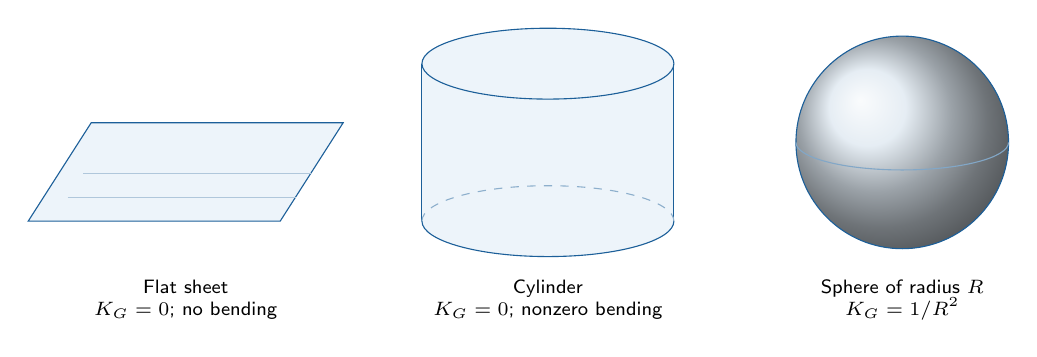
\begin{tikzpicture}
\begin{scope}
\fill[PaleBlue] (0,0)--(3.2,0)--(4,1.25)--(.8,1.25)--cycle;
\draw[KnownBlue] (0,0)--(3.2,0)--(4,1.25)--(.8,1.25)--cycle;
\draw[KnownBlue!35] (.5,.3)--(3.4,.3);
\draw[KnownBlue!35] (.7,.6)--(3.6,.6);
\node[lab] at (2,-1){Flat sheet\\$K_G=0$; no bending};
\end{scope}
\begin{scope}[shift={(5,0)}]
\fill[PaleBlue] (0,0) arc(180:360:1.6 and .45)--(3.2,2)
arc(0:180:1.6 and .45)--cycle;
\draw[KnownBlue] (0,0)--(0,2);
\draw[KnownBlue] (3.2,0)--(3.2,2);
\draw[KnownBlue] (1.6,2) ellipse(1.6 and .45);
\draw[KnownBlue] (0,0) arc(180:360:1.6 and .45);
\draw[KnownBlue!50,dashed] (0,0) arc(180:0:1.6 and .45);
\node[lab] at (1.6,-1){Cylinder\\$K_G=0$; nonzero bending};
\end{scope}
\begin{scope}[shift={(11.1,1)}]
\shade[ball color=KnownBlue!15] (0,0) circle(1.35);
\draw[KnownBlue] (0,0) circle(1.35);
\draw[KnownBlue!55] (-1.35,0) arc(180:360:1.35 and .35);
\node[lab] at (0,-2){Sphere of radius $R$\\$K_G=1/R^2$};
\end{scope}
\end{tikzpicture}
\end{center}
These are real-space teaching examples. A cylinder can be unrolled locally
without stretching: its intrinsic metric is flat, although it bends
in three dimensions. \textbf{Intrinsic} measurements use the surface metric;
\textbf{extrinsic} measurements also use an ambient space. \calc
\begin{knownbox}
\textbf{First fundamental form} is another name for the induced metric $g$.
\textbf{Second fundamental form} $II$ is the normal part of how tangent
directions change:
\[
\nabla_i^{\rm ambient}T_j
=\underbrace{\Gamma^k{}_{ij}T_k}_{\text{tangent part}}
 +\underbrace{II_{ij}}_{\text{normal part}}.
\qquad\text{\src{AP}{Appendix D, (D3)--(D5)}}
\]
For a surface, the Gauss equation says
\[
K_G=K_{\rm ambient}(T\Sigma)+
\frac{\langle II_{xx},II_{yy}\rangle-\|II_{xy}\|^2}{\det g}.
\]
\end{knownbox}
\begin{center}
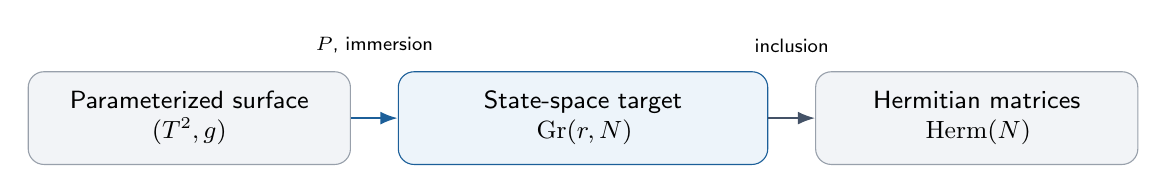
\begin{tikzpicture}
\node[basic,text width=3.6cm] (s) at (0,0)
{Parameterized surface\\$(T^2,g)$};
\node[known,text width=4.2cm] (g) at (5.0,0)
{State-space target\\$\Gr(r,N)$};
\node[basic,text width=3.6cm] (a) at (10.0,0)
{Hermitian matrices\\$\Herm(N)$};
\draw[flow] (s)--node[above=7mm,lab]{$P$, immersion}(g);
\draw[neutral,->] (g)--node[above=7mm,lab]{inclusion}(a);
\end{tikzpicture}
\end{center}
\textbf{Which ambient space?} The first map parameterizes the Bloch surface
and may have self-intersections. The second embeds the Grassmannian in
Hermitian matrices. Later, $II$ describes each regular image sheet
\emph{inside the Grassmannian}. The Grassmannian itself is curved inside the
flat matrix space. These are different second fundamental forms.
\begin{cautionbox}
A two-band regular patch locally fills $\CP^1$, so its $II$
\emph{inside $\CP^1$} vanishes. The sphere still bends inside the Hermitian
matrices. Thus $K_{II}=0$ does not mean that the sphere is flat.
Also, the unoccupied Hilbert subspace $Q\mathbb C^N$ is not the normal space
of the Bloch surface.
\end{cautionbox}

% PAGE 9: ONLY THE THREE PAPERS
\guidepage{8. The story told by the three papers}{A conceptual reading order: H1 $\rightarrow$ H2 $\rightarrow$ H3. It is not publication chronology.}
\begin{center}
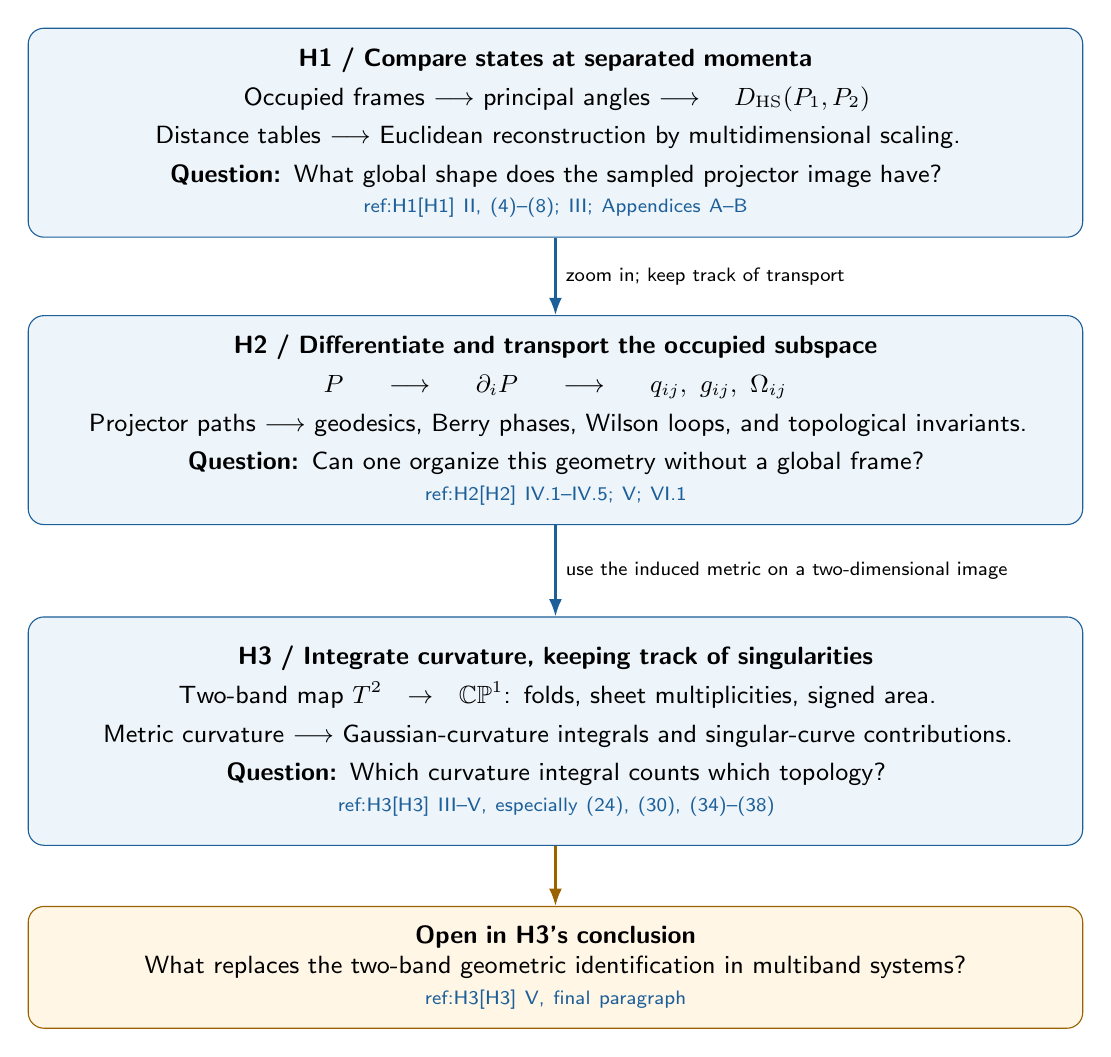
\begin{tikzpicture}
\node[known,text width=12.9cm,minimum height=2.5cm] (h1) at (0,0)
{\textbf{H1 / Compare states at separated momenta}\\[3pt]
Occupied frames $\longrightarrow$ principal angles
$\longrightarrow D_{\rm HS}(P_1,P_2)$\\[3pt]
Distance tables $\longrightarrow$ Euclidean reconstruction by
multidimensional scaling.\\[3pt]
\textbf{Question:} What global shape does the sampled projector image have?\\
\src{H1}{II, (4)--(8); III; Appendices A--B}};
\node[known,text width=12.9cm,minimum height=2.5cm] (h2) at (0,-3.65)
{\textbf{H2 / Differentiate and transport the occupied subspace}\\[3pt]
$P\longrightarrow \partial_iP\longrightarrow q_{ij},\ g_{ij},\ \Omega_{ij}$\\[3pt]
Projector paths $\longrightarrow$ geodesics, Berry phases, Wilson loops,
and topological invariants.\\[3pt]
\textbf{Question:} Can one organize this geometry without a global frame?\\
\src{H2}{IV.1--IV.5; V; VI.1}};
\node[known,text width=12.9cm,minimum height=2.9cm] (h3) at (0,-7.6)
{\textbf{H3 / Integrate curvature, keeping track of singularities}\\[3pt]
Two-band map $T^2\to\CP^1$: folds, sheet multiplicities, signed area.\\[3pt]
Metric curvature $\longrightarrow$ Gaussian-curvature integrals
and singular-curve contributions.\\[3pt]
\textbf{Question:} Which curvature integral counts which topology?\\
\src{H3}{III--V, especially (24), (30), (34)--(38)}};
\draw[flow] (h1.south)--node[right,lab]{zoom in; keep track of transport}(h2.north);
\draw[flow] (h2.south)--node[right,lab]{use the induced metric on a two-dimensional image}(h3.north);
\node[caution,text width=12.9cm] (open) at (0,-10.6)
{\textbf{Open in H3's conclusion}\\
What replaces the two-band geometric identification in multiband systems?\\
\src{H3}{V, final paragraph}};
\draw[->,CautionAmber,thick] (h3.south)--(open.north);
\end{tikzpicture}
\end{center}
\smallhead{What the three viewpoints add}
\textbf{H1: global comparison.} A distance table describes how far sampled
subspaces are from one another. A three-dimensional projection of its
reconstruction is a visualization of higher-dimensional data.

\textbf{H2: local calculus and transport.} Projectors provide a consistent
language for changing subspaces, including multiplets for which choosing
individual states is inconvenient.

\textbf{H3: careful global integration.} Signed and unsigned areas count
overlapping sheets differently. A smooth target does not guarantee a smooth
pullback metric on the Brillouin torus.

\begin{cautionbox}
Distances alone do not give an orientation. A plotted image also does not
automatically retain how often the source covers it.
H1 explicitly notes the orientation limitation. The multiband K\"ahler-angle
and complex-point analysis on later pages is a separate extension, not a
result attributed to these three papers.
\src{H1}{III.1.1, discussion after (11)}
\end{cautionbox}

% PAGE 10: FOLD AND SIGNED AREA
\guidepage{9. A fold is a failure of the map's derivative}{The Hamiltonian can stay gapped while one momentum direction stops changing the state.}
The simplest local fold is $f(s,t)=(s,t^2)$.
Two distinct points $(s,t)$ and $(s,-t)$ have the same image.
At $t=0$, the derivative in the $t$ direction vanishes.
\begin{center}
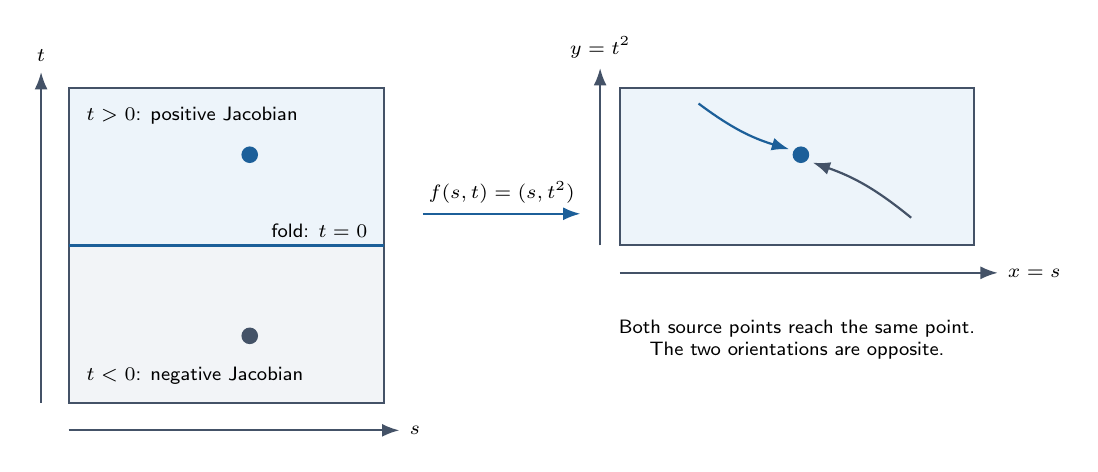
\begin{tikzpicture}
\fill[PaleBlue] (0,0) rectangle(4,2);
\fill[PaleGray] (0,-2) rectangle(4,0);
\draw[neutral] (0,-2) rectangle(4,2);
\draw[KnownBlue,very thick] (0,0)--(4,0);
\node[lab,anchor=west] at (.1,1.65){$t>0$: positive Jacobian};
\node[lab,anchor=west] at (.1,-1.65){$t<0$: negative Jacobian};
\draw[neutral,->] (0,-2.35)--(4.2,-2.35) node[right,lab]{$s$};
\draw[neutral,->] (-.35,-2)--(-.35,2.2) node[above,lab]{$t$};
\fill[KnownBlue] (2.3,1.15) circle(3pt);
\fill[Slate] (2.3,-1.15) circle(3pt);
\node[lab,anchor=west] at (2.45,.18){fold: $t=0$};
\draw[flow] (4.5,.4)--(6.5,.4) node[midway,above,lab]{$f(s,t)=(s,t^2)$};
\fill[PaleBlue] (7,0) rectangle(11.5,2);
\draw[neutral] (7,0) rectangle(11.5,2);
\draw[neutral,->] (7,-.35)--(11.8,-.35) node[right,lab]{$x=s$};
\draw[neutral,->] (6.75,0)--(6.75,2.25) node[above,lab]{$y=t^2$};
\fill[KnownBlue] (9.3,1.15) circle(3pt);
\draw[KnownBlue,->,thick] (8.0,1.8) to[bend right=10] (9.15,1.22);
\draw[Slate,->,thick] (10.7,.35) to[bend right=10] (9.45,1.05);
\node[lab] at (9.25,-1.2){Both source points reach the same point.\\The two orientations are opposite.};
\end{tikzpicture}
\end{center}
Using a flat target in this teaching example gives exactly
\[
g=\begin{pmatrix}1&0\\0&4t^2\end{pmatrix},\qquad
\dd A=2|t|\,\dd s\,\dd t,\qquad
\dd A_{\rm signed}=2t\,\dd s\wedge\dd t.
\quad\calc
\]
H3's target is a sphere rather than this flat plane; the rank-loss and
sheet-orientation mechanism is the same.
\src{H3}{III.1, Fig.\ 3}
\begin{knownbox}
\textbf{For a two-band map, in this guide's convention:}
\[
U=\{\mathbf k\in T^2:\det g(\mathbf k)>0\}.
\]
\[
\sqrt{\det g}=\frac{|\Omega_{xy}|}{2},\qquad K_G=4,
\qquad
\frac1{4\pi}\int_U K_G\,\operatorname{sgn}(\Omega_{xy})\,\dd A=C.
\]
\src{R}{IIA, (41), with the chain rule}\quad
\src{H3}{IV, (37), converted conventions}
\end{knownbox}
On $U$, the signed curvature density is $2\Omega$; it extends by zero across
the critical set, where $\Omega=0$. This assigns no ordinary Gaussian
curvature to the degenerate metric there.
\textbf{Unsigned area} counts every sheet positively. \textbf{Signed area}
counts positive and negative sheets with opposite signs. The signed formula
above is a degree identity. It is not ordinary Gauss--Bonnet for a smooth
torus metric.

\textbf{Singular curvature.} Cutting along the fold produces boundaries.
Their turning supplies an additional curve contribution.
H3's example uses a bulk integral plus twice the fold-curve integral in its
generalized Gauss--Bonnet formula. Its unsigned bulk value divided by
$2\pi$ is about $2.3779$, while the fold contribution compensates it.
\src{H3}{III.3; IV, (30), (34)}
\begin{cautionbox}
A globally immersive $T^2\to S^2$ would be a covering of the sphere, which a
torus cannot be. Some rank loss is unavoidable for a smooth two-band map.
Generic folds can have cusp points; other special maps have branch points.
A particular four-cusp formula should not be applied to every singular map.
\src{MO}{Theorem 3}\quad\src{H3}{IV, (35)--(36), specific configuration}
\end{cautionbox}

% PAGE 11: KAHLER ANGLE
\guidepage{10. The missing angle in a multiband system}{The next pages explain the proposed extension [E] using established geometric ingredients.}
\textbf{Complex structure $J$.} On a complex vector space, multiplication by
$\ii$ is a real-linear operation with $J^2=-I$. It rotates a direction through
$90^\circ$ in its complex line. Here it acts on \emph{state-change vectors}
$B$, not on the arbitrary overall phase of $\ket u$.

\textbf{K\"ahler structure.} The Grassmannian has a compatible metric $G$,
complex structure $J$, and closed area-like two-form $\omega$:
$\omega(X,Y)=G(JX,Y)$ and $\nabla J=0$.
The induced quantum metric and Berry curvature are their pullbacks, up to
the fixed factor and orientation convention.
\src{MO}{II; Appendix A}

Choose $e_1,e_2$ as an orthonormal basis of the image tangent plane, with
the orientation induced by the ordered momentum directions
$(\partial_x,\partial_y)$.
\begin{center}
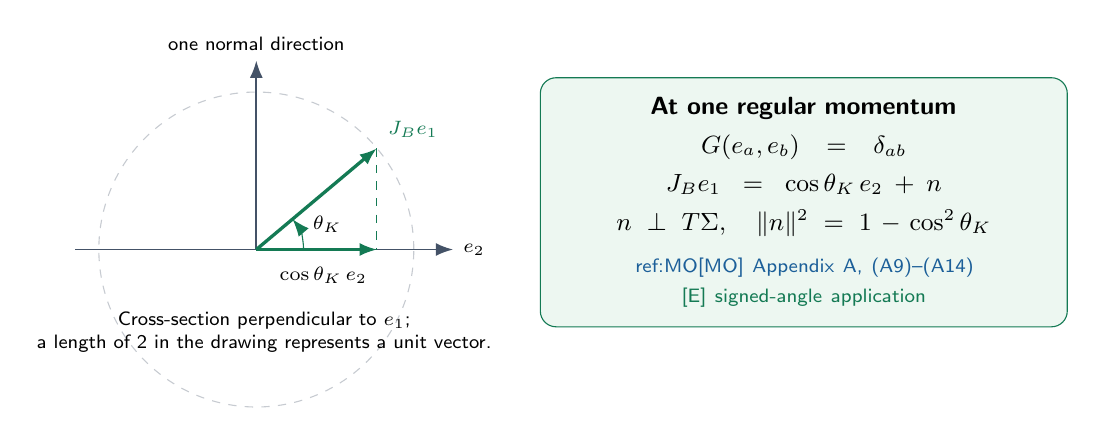
\begin{tikzpicture}
\begin{scope}[shift={(2.6,0)}]
\draw[Slate!30,dashed] (0,0) circle(2);
\draw[neutral,->] (-2.3,0)--(2.5,0) node[right,lab]{$e_2$};
\draw[neutral,->] (0,0)--(0,2.4) node[above,lab]{one normal direction};
\draw[ProposalGreen,->,very thick] (0,0)--(1.532,1.286)
 node[above right,lab]{$J_Be_1$};
\draw[ProposalGreen,dashed] (1.532,1.286)--(1.532,0);
\draw[ProposalGreen,->,thick] (0,0)--(1.532,0);
\node[lab,anchor=north] at (.85,-.1){$\cos\theta_K\,e_2$};
\draw[ProposalGreen,->] (.6,0) arc(0:40:.6);
\node[lab] at (.9,.32){$\theta_K$};
\node[lab] at (.1,-1.05){Cross-section perpendicular to $e_1$;\\a length of 2 in the drawing represents a unit vector.};
\end{scope}
\node[proposed,text width=6.2cm,anchor=west] at (6.2,.6)
{\textbf{At one regular momentum}\\[3pt]
$G(e_a,e_b)=\delta_{ab}$\\[3pt]
$J_Be_1=\cos\theta_K\,e_2+n$\\[3pt]
$n\perp T\Sigma,\quad\|n\|^2=1-\cos^2\theta_K$\\[4pt]
\src{MO}{Appendix A, (A9)--(A14)}\\
\esrc{signed-angle application}};
\end{tikzpicture}
\end{center}
\begin{extensionbox}
Choose the Berry-compatible complex structure $J_B$ and define
\[
\boxed{\cos\theta_K=\frac{\Omega_{xy}}{2\sqrt{\det g}}},\qquad
\Omega_{xy}\,\dd k_x\dd k_y=2\cos\theta_K\,\dd A.
\]
Berry curvature is quantum area weighted by the alignment of the tangent
plane with the complex structure.
\esrc{interpretation of the K\"ahler pullback framework}
\end{extensionbox}
\begin{tabularx}{\linewidth}{@{}p{2.1cm}p{3.4cm}X@{}}
\toprule
$\theta_K$ & Tangent-plane relation & Physical geometric statement\\
\midrule
$0$ or $\pi$ & Complex line & $|\Omega|=2\sqrt{\det g}$: determinant saturation.\\
$\pi/2$ & Isotropic plane & $\Omega=0$; the state can still change in two independent directions.\\
Intermediate & Partial alignment & $0<|\Omega|<2\sqrt{\det g}$.\\
\bottomrule
\end{tabularx}
\smallskip
\textbf{The viewpoint.} A sphere has no extra tangent-space direction into
which $J_Be_1$ can leave the image plane. A higher-dimensional target does.
This is why area and Berry curvature separate beyond two bands.
\begin{cautionbox}
The angle requires $\det g>0$. It describes one tangent plane, not its rate
of bending. With the usual holomorphic $J_0$, $J_B=-J_0$ and
$P^*\omega_{\rm FS}=-\Omega/2$; the sign of the cosine reverses.
Absolute values and saturation do not depend on this choice.
\src{MO}{II; Appendix A}
\end{cautionbox}

% PAGE 12: WEDGE
\guidepage{11. A wedge tests complex independence}{The algebra is a Gram determinant; the new use is its band-geometric interpretation.}
For a rank-one band, treat $B_x$ and $B_y$ as complex vectors in
$\mathbb C^{N-1}$ and write $z=B_x^\dagger B_y$. Then
\[
\det g=\|B_x\|^2\|B_y\|^2-(\Ree z)^2,\qquad
\frac{\Omega_{xy}^2}{4}=(\Imm z)^2.
\]
The squared complex-wedge norm is
$\|B_x\wedge B_y\|^2=\|B_x\|^2\|B_y\|^2-|z|^2$.
Subtract the two expressions to obtain
\begin{extensionbox}
\[
\boxed{\det g=\frac{\Omega_{xy}^2}{4}+\|B_x\wedge B_y\|^2.}
\]
\esrc{application}\quad\calc\quad
\src{MO}{Appendix A, determinant inequality and equality condition}
\end{extensionbox}
\textbf{Wedge product.} A generalized oriented area, with a useful algebraic
test: $B_x\wedge B_y=0$ exactly when the vectors are complex linearly dependent.
It need not vanish when they are merely nonorthogonal.

\smallhead{A two-number example that separates all three cases}
Take $B_x=(1,0)$ and $B_y=(\ii a,b)$, with real $a,b$:
\[
g=\begin{pmatrix}1&0\\0&a^2+b^2\end{pmatrix},\qquad
\Omega_{xy}=-2a,\qquad \|B_x\wedge B_y\|^2=b^2.
\quad\calc
\]
\begin{center}
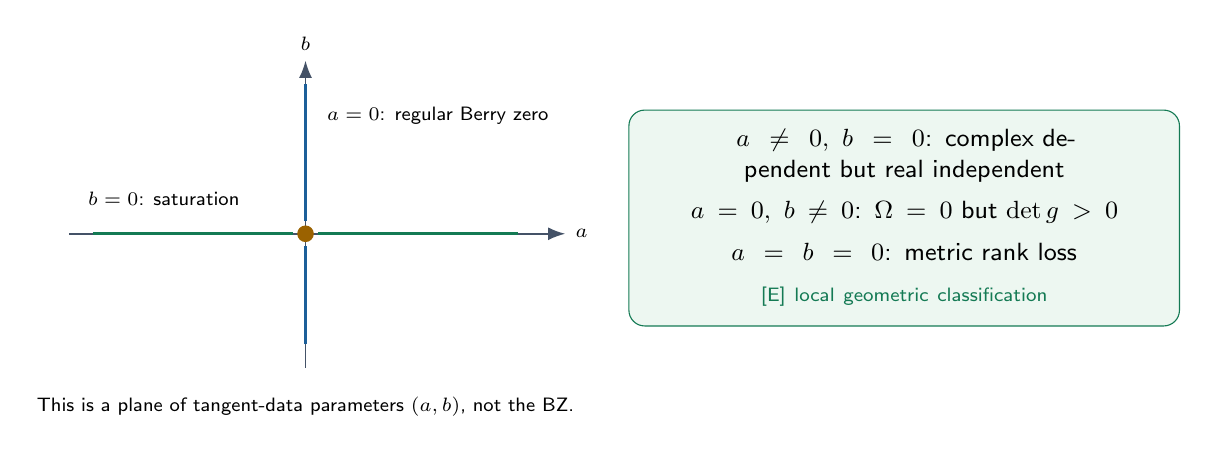
\begin{tikzpicture}
\draw[neutral,->] (-3,0)--(3.3,0) node[right,lab]{$a$};
\draw[neutral,->] (0,-1.7)--(0,2.2) node[above,lab]{$b$};
\draw[ProposalGreen,very thick] (-2.7,0)--(-.16,0);
\draw[ProposalGreen,very thick] (.16,0)--(2.7,0);
\draw[KnownBlue,very thick] (0,.16)--(0,1.9);
\draw[KnownBlue,very thick] (0,-1.4)--(0,-.16);
\fill[CautionAmber] (0,0) circle(3pt);
\node[lab] at (-1.8,.45){$b=0$: saturation};
\node[lab,anchor=west] at (.15,1.5){$a=0$: regular Berry zero};
\node[lab,anchor=north] at (0,-1.95){This is a plane of tangent-data parameters $(a,b)$, not the BZ.};
\node[proposed,text width=6.5cm,anchor=west] at (4.1,.2)
{$a\ne0,\ b=0$: complex dependent but real independent\\[4pt]
$a=0,\ b\ne0$: $\Omega=0$ but $\det g>0$\\[4pt]
$a=b=0$: metric rank loss\\[4pt]
\esrc{local geometric classification}};
\end{tikzpicture}
\end{center}
\textbf{Why complex dependence need not collapse area.}
The vectors $B_x$ and $\ii B_x$ are dependent over $\mathbb C$, but independent
over $\mathbb R$. They span a genuine real plane. The metric tests real
independence; the wedge above tests complex independence.

\textbf{A real physical-state example of regular Berry zero.}
On a local momentum patch,
\[
\ket{u(x,y)}=\frac{(1,x,y)^T}{\sqrt{1+x^2+y^2}}
\quad\Longrightarrow\quad
\Omega_{xy}=0,\qquad \det g=(1+x^2+y^2)^{-3}>0.
\]
The normalized state is real and still changes in two independent directions.
This local three-band example is an explicit calculation, not a periodic
Chern-insulator model. \calc

% PAGE 13: HIERARCHY
\guidepage{12. Why two, three, and more bands differ}{A genericity statement for one occupied band, not a prohibition on special models.}
For one occupied band, the target $\CP^{N-1}$ has complex dimension $N-1$.
A two-dimensional Brillouin zone samples real tangent planes in that target.
Requiring such a plane to be a complex line imposes more conditions as the
target dimension increases.
\src{MO}{Appendix A, complex-tangent criterion}\quad\esrc{dimension-counting application}
\begin{center}
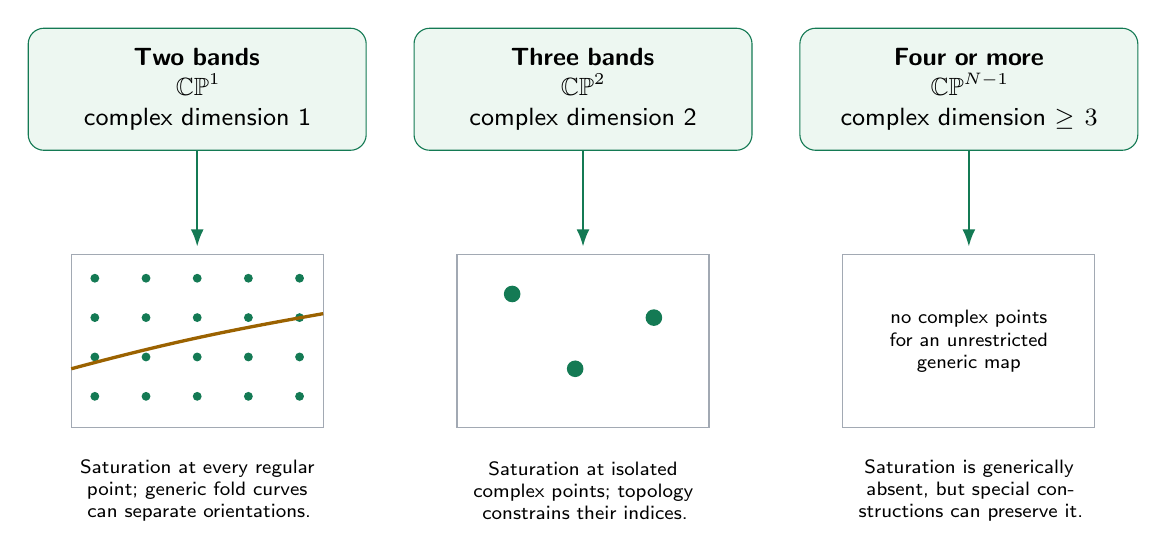
\begin{tikzpicture}
\node[proposed,text width=3.8cm,minimum height=1.55cm] (a) at (0,0)
{\textbf{Two bands}\\$\CP^1$\\complex dimension 1};
\node[proposed,text width=3.8cm,minimum height=1.55cm] (b) at (4.9,0)
{\textbf{Three bands}\\$\CP^2$\\complex dimension 2};
\node[proposed,text width=3.8cm,minimum height=1.55cm] (c) at (9.8,0)
{\textbf{Four or more}\\$\CP^{N-1}$\\complex dimension $\ge3$};
\foreach \x in {0,4.9,9.8}{
 \draw[Slate!50] (\x-1.6,-2.1) rectangle(\x+1.6,-4.3);
}
\foreach \xx in {-1.3,-.65,0,.65,1.3}{
 \foreach \yy in {-2.4,-2.9,-3.4,-3.9}{
 \fill[ProposalGreen] (\xx,\yy) circle(1.6pt);
 }}
\draw[CautionAmber,very thick] (-1.6,-3.55) to[out=15,in=190] (1.6,-2.85);
\foreach \x/\y in {4.0/-2.6,4.8/-3.55,5.8/-2.9}{
 \fill[ProposalGreen] (\x,\y) circle(3pt);
}
\node[lab] at (9.8,-3.2){no complex points\\for an unrestricted\\generic map};
\draw[eflow] (a.south)--(0,-2.0);
\draw[eflow] (b.south)--(4.9,-2.0);
\draw[eflow] (c.south)--(9.8,-2.0);
\node[lab,text width=3.9cm] at (0,-5.1)
{Saturation at every regular point; generic fold curves can separate orientations.};
\node[lab,text width=3.9cm] at (4.9,-5.1)
{Saturation at isolated complex points; topology constrains their indices.};
\node[lab,text width=3.9cm] at (9.8,-5.1)
{Saturation is generically absent, but special constructions can preserve it.};
\end{tikzpicture}
\end{center}
The rectangles are schematic BZ patches. Green dots indicate saturation;
they are not numerical root positions. In the middle panel, the number drawn
illustrates discreteness and is not a universal exact count.

\begin{extensionbox}
\textbf{The dimension count.} If the target has complex dimension $m$,
the complex-line locus inside the real two-plane Grassmannian has real
codimension $2m-2$. A two-dimensional source generically meets:
\[
\begin{array}{c|ccc}
m & 1 & 2 & \ge3\\ \hline
\text{codimension} &0&2&\ge4\\
\text{saturation locus} &\text{all regular points}&\text{isolated}&\text{empty}
\end{array}
\]
Rank-deficient derivatives have codimension $2m-1$, explaining why generic
three-band maps avoid folds. \esrc{transversality/dimension reasoning}
\end{extensionbox}

\textbf{Generic means stable expectation under unrestricted small smooth
perturbations.} It does not mean every Hamiltonian in that band count.
Symmetries or a construction confined to a smaller target can change the result.
\begin{cautionbox}
\[
P(\mathbf k)\longmapsto P(\mathbf k)\oplus 0
\]
adds a decoupled orbital and leaves $g$, $\Omega$, and saturation unchanged.
Therefore higher band number cannot, by itself, forbid ideality or complex
points. For occupied rank $r$, use $m=r(N-r)$; the table above was stated for
$r=1$. \calc
\end{cautionbox}

% PAGE 14: COMPLEX POINT INDEX
\guidepage{13. Why three bands carry a signed zero count}{A line bundle can force a section to vanish. This is the most advanced conceptual step.}
Let $L$ be the occupied line bundle of a three-band system.
The two derivatives are maps $B_i:L\to L^\perp$.
Their wedge is a section of a complex line bundle:
\[
W=B_x\wedge B_y
\in\Gamma\!\left(\Lambda^2 L^\perp\otimes(L^*)^{\otimes2}\right).
\]
Here $\Lambda^2$ takes the determinant line of the two-dimensional empty
space; $L^*$ is the dual line; $\Gamma$ means the collection of smooth sections.
\esrc{bundle construction}
\begin{center}
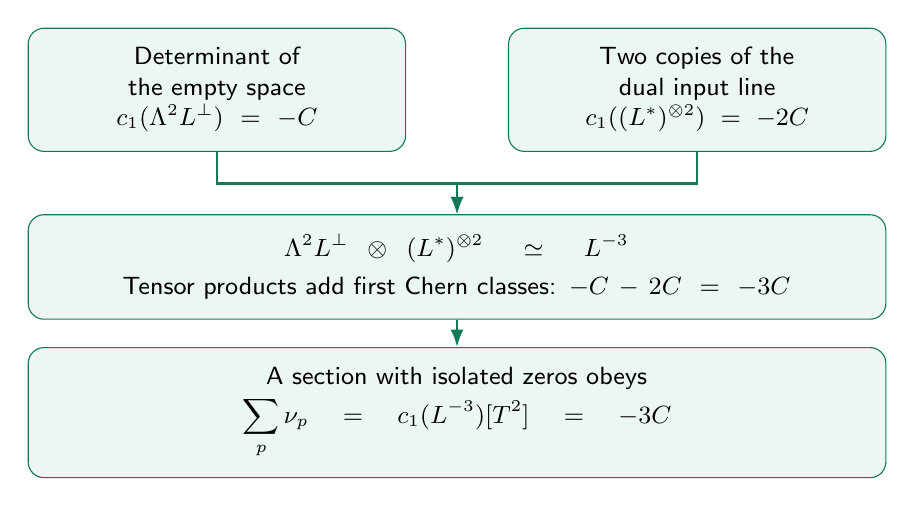
\begin{tikzpicture}
\node[proposed,text width=4.3cm] (q) at (0,0)
{Determinant of the empty space\\
$c_1(\Lambda^2 L^\perp)=-C$};
\node[proposed,text width=4.3cm] (l) at (6.1,0)
{Two copies of the dual input line\\
$c_1((L^*)^{\otimes2})=-2C$};
\node[proposed,text width=10.4cm] (w) at (3.05,-2.25)
{$\Lambda^2L^\perp\otimes(L^*)^{\otimes2}\simeq L^{-3}$\\[3pt]
Tensor products add first Chern classes: $-C-2C=-3C$};
\draw[eflow] (q.south)--++(0,-.4)-|(w.north);
\draw[eflow] (l.south)--++(0,-.4)-|(w.north);
\node[proposed,text width=10.4cm] (z) at (3.05,-4.1)
{A section with isolated zeros obeys\\[2pt]
$\displaystyle \sum_p\nu_p=c_1(L^{-3})[T^2]=-3C$};
\draw[eflow] (w)--(z);
\end{tikzpicture}
\end{center}
\textbf{Why the empty-space class is $-C$.}
The full orbital bundle is trivial in the fixed periodic basis:
$L\oplus L^\perp=T^2\times\mathbb C^3$. Its total first Chern class is zero.
The dual changes the sign; tensor powers multiply the class.
\esrc{elementary bundle derivation}\quad\src{F}{(1.1), for the complex-point connection}

\textbf{Local winding index.} Choose a gauge smooth on a disk around one zero.
The phase of the local complex number representing $W$ winds by $2\pi\nu_p$
around the disk boundary. For a simple zero, $\nu_p=\pm1$.
\begin{center}
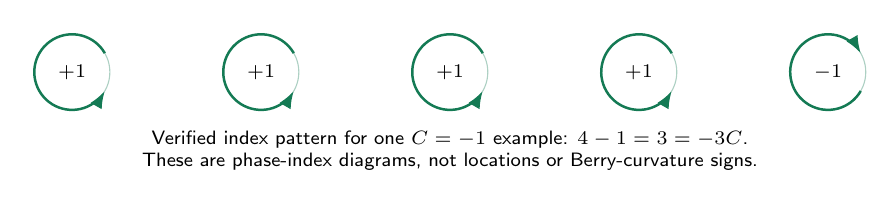
\begin{tikzpicture}
\foreach \x in {0,2.4,4.8,7.2}{
 \draw[ProposalGreen!35] (\x,0) circle(.48);
 \draw[eflow] (\x+.416,.24) arc(30:330:.48);
 \node[lab] at (\x,0){$+1$};
}
\draw[ProposalGreen!35] (9.6,0) circle(.48);
\draw[eflow] (10.016,-.24) arc(-30:-330:.48);
\node[lab] at (9.6,0){$-1$};
\node[lab] at (4.8,-1.0)
{Verified index pattern for one $C=-1$ example: $4-1=3=-3C$.\\
These are phase-index diagrams, not locations or Berry-curvature signs.};
\end{tikzpicture}
\end{center}
\begin{extensionbox}
For an immersion with simple zeros,
\[
\boxed{N_{\rm complex}=3|C|+2\ell,\qquad \ell=0,1,2,\ldots .}
\]
Topology fixes the signed sum, not the exact unsigned number.
Without simple zeros, a single zero can carry higher multiplicity.
\esrc{index consequence; five roots independently confirmed in the supplied example}
\end{extensionbox}
The relation is a band-language instance of the classical Lai formulas.
Here $I_+$ and $I_-$ sum the local Bishop indices at complex points whose
tangent orientation agrees or disagrees with the usual holomorphic
structure $J_0$. They obey
\[
I_+-I_-=-3C,\qquad I_++I_-=\chi(T^2)+e(\nu).
\]
The winding of $W$ equals the Bishop index at a $J_0$-positive complex point
and its negative at a $J_0$-negative point. Thus the subscripts on $I_\pm$
specify complex-point orientation, not the sign of the $W$-winding.
Here $e(\nu)$ is the Euler number of the normal bundle.
\src{L}{classical index theorem}\quad\src{F}{(1.1)}

% PAGE 15: GAUSS EQUATION / TOPOLOGY
\guidepage{14. Where the multiband Gaussian curvature comes from}{One part belongs to the Grassmannian; another comes from the Bloch surface's bending.}
\begin{extensionbox}
\[
\boxed{K_G=K_{\Gr}+K_{II}},\qquad
K_{II}=
\frac{\langle II_{xx},II_{yy}\rangle-\|II_{xy}\|^2}{\det g}.
\]
Here every inner product uses $G(A,B)=\frac12\Ree\Tr(A^\dagger B)$.
\src{AP}{Appendix D, Gauss equation}\quad\esrc{projector specialization}
\end{extensionbox}
Define anti-Hermitian curvature blocks
\[
\mathcal F_o=P[\partial_xP,\partial_yP]P,\qquad
\mathcal F_u=Q[\partial_xP,\partial_yP]Q.
\]
Their norms determine the ambient sectional curvature of the image tangent
plane:
\[
\boxed{K_{\Gr}=
\frac{\|\mathcal F_o\|_F^2+\|\mathcal F_u\|_F^2}{2\det g}.}
\qquad\esrc{Grassmann quotient curvature; Appendix A below}
\]
For rank one, this becomes $K_{\Gr}=1+3\cos^2\theta_K$.
For higher rank, the traced scalar $\Omega=\ii\Tr\mathcal F_o$ does not
determine both matrix norms. The bending term can be negative.
Ambient sectional curvature is nonnegative in general; in the rank-one case
it lies between $1$ and $4$.

\begin{center}
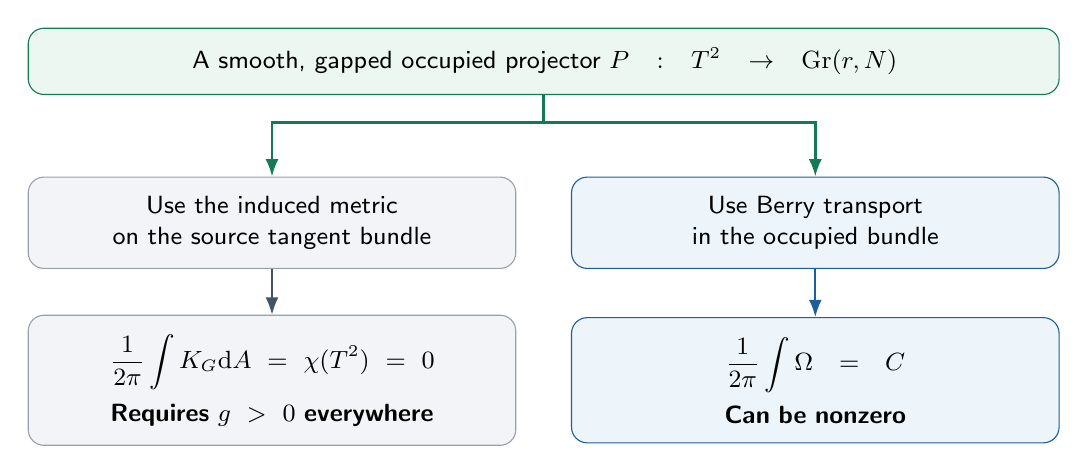
\begin{tikzpicture}
\node[proposed,text width=12.6cm] (p) at (0,0)
{A smooth, gapped occupied projector $P:T^2\to\Gr(r,N)$};
\node[basic,text width=5.7cm] (g) at (-3.45,-2.05)
{Use the induced metric\\
on the source tangent bundle};
\node[known,text width=5.7cm] (b) at (3.45,-2.05)
{Use Berry transport\\
in the occupied bundle};
\node[basic,text width=5.7cm] (ga) at (-3.45,-4.05)
{$\displaystyle\frac1{2\pi}\int K_G\dd A=\chi(T^2)=0$\\[4pt]
\textbf{Requires $g>0$ everywhere}};
\node[known,text width=5.7cm] (bc) at (3.45,-4.05)
{$\displaystyle\frac1{2\pi}\int\Omega=C$\\[4pt]
\textbf{Can be nonzero}};
\draw[eflow] (p.south)--++(0,-.35)-|(g.north);
\draw[eflow] (p.south)--++(0,-.35)-|(b.north);
\draw[neutral,->] (g)--(ga);
\draw[flow] (b)--(bc);
\end{tikzpicture}
\end{center}
\textbf{The viewpoint.} The two integrals concern different bundles.
Ordinary total Gaussian curvature measures the topology of the source
surface. The Chern number measures the occupied-state bundle.
This does not remove other restrictions between metric and topology, such as
the volume bound $\int\dd A\ge\pi|C|$.
\src{MO}{Theorem 2}\quad\esrc{Gauss--Bonnet interpretation}

\textbf{Evidence in the supplied study.}
The three-band rank-one and four-band rank-two models have $C=-1$ and $-2$.
Their Gauss-equation curvature agrees with a metric-only Brioschi calculation
under grid refinement, and their total Gaussian-curvature integrals converge
to zero. The two-band control retains constant regular curvature.
\esrc{independent numerical checks in the earlier verification archive}
\begin{cautionbox}
A gap ensures a smooth projector; it does not prove $g>0$.
Finite grids provide evidence of immersion, not a global proof.
These results address smooth Hermitian immersion geometry.
A universal treatment of singular multiband maps or a new response involving
$K_{II}$ requires additional work.
\end{cautionbox}

% PAGE 16: OBSERVABLES
\guidepage{15. Where the geometry meets familiar physics}{The review supplies the response context; a geometric invariant is not automatically a new observable.}
For $m\ne n$, an interband dipole matrix element is
\[
r^a_{mn}=\ii\langle u_m|\partial_a u_n\rangle.
\]
It describes how light polarized along $a$ couples the two bands.
The review packages it as an operator-valued tangent vector
$\hat e_a^{mn}=r^a_{mn}\ket{u_m}\bra{u_n}$.
\src{R}{IIIH, (312)--(314), pp.\ 27--28}
\begin{center}
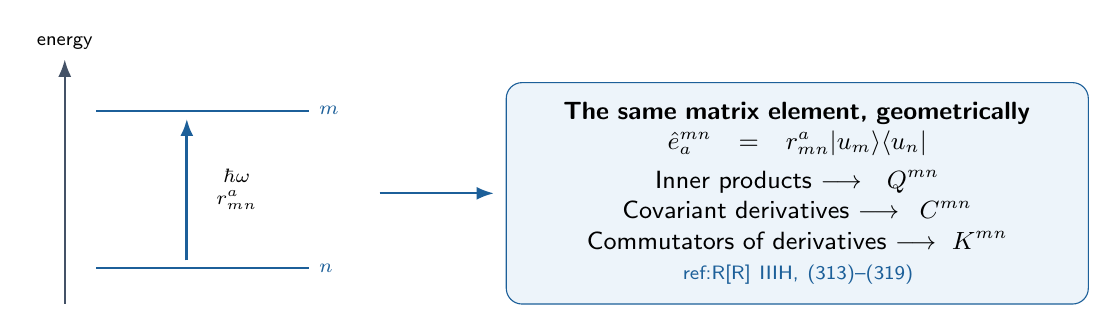
\begin{tikzpicture}
\draw[neutral,->] (0,0)--(0,3.1) node[above,lab]{energy};
\draw[KnownBlue,thick] (.4,.45)--(3.1,.45) node[right,lab]{$n$};
\draw[KnownBlue,thick] (.4,2.45)--(3.1,2.45) node[right,lab]{$m$};
\draw[KnownBlue,->,very thick] (1.55,.55)--(1.55,2.35);
\node[lab,anchor=west] at (1.8,1.45){$\hbar\omega$\\$r^a_{mn}$};
\draw[flow] (4.0,1.4)--(5.45,1.4);
\node[known,text width=6.9cm,anchor=west] at (5.6,1.4)
{\textbf{The same matrix element, geometrically}\\
$\hat e_a^{mn}=r^a_{mn}\ket{u_m}\bra{u_n}$\\[3pt]
Inner products $\longrightarrow Q^{mn}$\\
Covariant derivatives $\longrightarrow C^{mn}$\\
Commutators of derivatives $\longrightarrow K^{mn}$\\
\src{R}{IIIH, (313)--(319)}};
\end{tikzpicture}
\end{center}
\begin{tabularx}{\linewidth}{@{}p{4.1cm}X@{}}
\toprule
Physical question & Relation and scope in the review\\
\midrule
Intrinsic Hall response &
The occupied-state Berry curvature enters the Hall conductivity.
\src{R}{IIIC, (218), p.\ 19}\\[5pt]
Linear optical absorption &
Band-pair inner products $Q^{mn}$ enter a resonant, occupation-weighted
integral. \src{R}{IIIH, (320), p.\ 28}\\[5pt]
Shift current &
Covariant derivatives of transition elements enter through $C^{mn}$.
\src{R}{IIIH, (321), p.\ 28}\\[5pt]
Third-order injection &
One contribution contains the optical curvature tensor $K^{mn}$.
Other terms are present. \src{R}{IIIH, (323), p.\ 28}\\[5pt]
Momentum-resolved geometry &
ARPES-based reconstructions include energy-weighted quasi-QGTs and
model-dependent conversion steps.
\src{R}{VD, (340)--(342), pp.\ 50--51}\\
\bottomrule
\end{tabularx}
\smallhead{A concrete covariant derivative}
A transition amplitude acquires the relative phase of its initial and final
states. Its derivative must therefore include their connection difference:
\[
D_c r^a_{mn}=\partial_c r^a_{mn}
-\ii(A_{m,c}-A_{n,c})r^a_{mn}.
\quad\src{R}{IIIH, (318)}
\]
This is a direct physics example of correcting for a changing local frame.

\begin{cautionbox}
\textbf{The objects called curvature are different.}
The optical construction uses band pairs and a flag-manifold viewpoint
$U(N)/U(1)^N$. Its $K^{mn}$ is not automatically the Gaussian curvature of
one band's two-dimensional quantum metric, or the scalar $K_{II}$.
\src{R}{Fig.\ 3 and (319), p.\ 28}
\end{cautionbox}
\begin{extensionbox}
\textbf{What the extension would let you reconstruct.}
If the full $g_{ij}(\mathbf k)$ and $\Omega_{xy}(\mathbf k)$ are available
on a region where $\det g>0$, then
$\cos\theta_K=\Omega/(2\sqrt{\det g})$ follows directly.
Locating regular determinant-saturation points is then meaningful.
A specific new response proportional to $K_{II}$ is not established here.
\esrc{operational interpretation, with the measurement assumptions retained}
\end{extensionbox}

% PAGE 17: DICTIONARY
\guidepage{16. Dictionary: each word has a physics anchor}{Use this as an index after reading the pictures, rather than memorizing the definitions first.}
\renewcommand{\arraystretch}{1.19}
{\small
\begin{tabularx}{\linewidth}{@{}>{\raggedright\arraybackslash}p{3.15cm}Xr@{}}
\toprule
Term & Familiar object or operational picture & Page\\
\midrule
Parameter manifold & The set of momenta or control parameters. &2\\
Coordinate chart & A local choice of labels, such as $\theta,\phi$. &2,6\\
Ray & All vectors representing the same pure physical state. &2\\
Projective space & The set of rays; two levels give the Bloch sphere. &2\\
Projector & A gauge-independent matrix encoding a state/subspace. &2--3\\
Frame / gauge & The basis or phase representatives used locally. &3,7\\
Grassmannian & The set of occupied $r$-planes in $\mathbb C^N$. &3\\
Vector bundle / fiber & The occupied vector space attached to each $\mathbf k$. &3\\
Section & A smoothly chosen vector in each fiber; zeros are allowed. &3,14\\
Principal angle & A basis-independent angle between two subspaces. &4\\
Geodesic & A locally straight path; sufficiently short segments minimize length. &4\\
Pullback & Measure $\dd P$ and assign that length rule to $\dd\mathbf k$. &4\\
Tangent vector & A first-order state/subspace change, $\partial_iP$. &5,8\\
Quantum metric & The real Gram matrix of physical state changes. &4--6\\
Berry connection & A local rule for phase or occupied-frame transport. &7\\
Holonomy / Wilson loop & The transformation remaining after a closed trip. &7\\
Covariant derivative & A derivative corrected for changing local frames. &7,16\\
Christoffel symbols & Coefficients describing change of a tangent basis. &7\\
Immersion / fold & Independent tangent directions / the simple rank-loss model $(s,t)\mapsto(s,t^2)$. &8,10\\
Normal / second form & Directions away from the surface / its bending. &8,15\\
Gaussian curvature & The intrinsic curvature of a two-dimensional metric. &6--8\\
Sectional curvature & Ambient curvature assigned to one tangent two-plane. &15\\
Complex structure & Multiplication by $\ii$ on state-change directions. &11\\
K\"ahler angle & Alignment of a real tangent plane with its complex rotation. &11\\
Wedge / complex point & Complex independence test / saturation at an immersion. &12--14\\
Chern number / Euler characteristic & $C$ concerns the occupied bundle; $\chi(\Sigma)$ concerns the source surface. &7,15\\
\bottomrule
\end{tabularx}}
\renewcommand{\arraystretch}{1}
\begin{plainbox}
\textbf{The central dependency chain}
\[
\text{state}\ \longrightarrow\ P\ \longrightarrow\ \dd P
\ \longrightarrow\ q=g-\frac{\ii}{2}\Omega
\ \longrightarrow\ \text{local geometry}.
\]
Then split the questions: compare states; transport states; transport tangent
arrows; bend a surface; integrate a curvature. Each operation uses a
specific object and a specific space.
\end{plainbox}

% PAGE 18: CONVENTIONS
\guidepage{17. A convention ledger for reading the papers}{The guide fixes one convention so the pictures and formulas can be checked against each other.}
\begin{knownbox}
\[
A_i=\ii\langle u|\partial_i u\rangle,\qquad
\Omega_{xy}=\ii\Tr\!\left(P[\partial_xP,\partial_yP]\right),
\qquad q_{ij}=g_{ij}-\frac{\ii}{2}\Omega_{ij}.
\]
\[
g_{ij}=\tfrac12\Tr(\partial_iP\,\partial_jP),\qquad
\dd A=\sqrt{\det g}\,\dd k_x\dd k_y,\qquad
C=\tfrac1{2\pi}\int\Omega.
\]
\src{R}{IIA, (4), (7), (11)--(14)}\quad
\src{H2}{IV.2, (27)--(30), after metric rescaling}
\end{knownbox}
\begin{tabularx}{\linewidth}{@{}>{\raggedright\arraybackslash}p{4.1cm}XX@{}}
\toprule
Quantity & This guide / standard & Huang's doubled metric\\
\midrule
Metric & $g$ & $g_H=2g$\\[4pt]
Length & $\dd s$ & $\dd s_H=\sqrt2\,\dd s$\\[4pt]
Area in two dimensions & $\dd A$ & $\dd A_H=2\,\dd A$\\[4pt]
Gaussian curvature & $K_G$ & $K_{G,H}=K_G/2$\\[4pt]
Regular two-band sphere & $R=1/2,\ K_G=4$ & $R_H=1/\sqrt2,\ K_{G,H}=2$\\[4pt]
Integrated curvature & $K_G\dd A$ & Unchanged\\
\bottomrule
\end{tabularx}
\smallskip
\src{H2}{IV.2, (27)}\quad\src{H3}{II.2, (2)}\quad\calc

\smallhead{One sign difference between the papers}
H2 uses $\Omega=\ii\Tr(P[\partial_xP,\partial_yP])$.
H3 defines its signed density by the opposite sign in Eq.\ (24), then calls
it Berry curvature in Eq.\ (38). For identical $P$ and coordinate orientation:
\[
\Omega_{\mathrm{H3}}=-\Omega_{\mathrm{H2}},
\qquad C_{\mathrm{H3}}=-C_{\mathrm{H2}}.
\]
This is separate from the metric's factor of two. The guide converts both
when discussing H3's signed integral.
\src{H2}{(29)}\quad\src{H3}{(24), (38)}

\smallhead{Two operations with the same letter are not necessarily the same}
\begin{tabularx}{\linewidth}{@{}>{\raggedright\arraybackslash}p{3.2cm}X@{}}
\toprule
Symbol in this guide & Meaning\\
\midrule
$\Omega_{xy}$ & Scalar Berry-curvature component; $\Omega=\Omega_{xy}\dd k_x\wedge\dd k_y$ is the two-form.\\[4pt]
$\mathcal F_o,\mathcal F_u$ & Matrix-valued anti-Hermitian curvature blocks; $\ii\Tr\mathcal F_o=\Omega_{xy}$.\\[4pt]
$K_G,\ K_{\Gr}$ & Source-metric Gaussian curvature; ambient Grassmann sectional curvature.\\[4pt]
$K^{mn}$ in the review & Optical band-pair curvature, with its own definition.\\[4pt]
$G,\ g$ & Metric on the target; metric pulled back to the Brillouin zone.\\
\bottomrule
\end{tabularx}

\begin{cautionbox}
H2's $-\tfrac14[[X,Y],Z]$ formula in III.2 is for the unitary group $U(N)$.
Its coefficient is not the Grassmann quotient coefficient.
The direct projector/Gauss derivation on page 21 avoids that substitution.
Also, read the sphere radius from its metric: $g_H=\tfrac12\dd\mathbf n^2$
has radius $1/\sqrt2$, regardless of the inconsistent radius stated in H3's prose.
\end{cautionbox}

% PAGE 19: STUDY ROUTE
\guidepage{18. A manageable learning route}{The goal is to recognize the object being measured before learning the theorem's name.}
\begin{center}
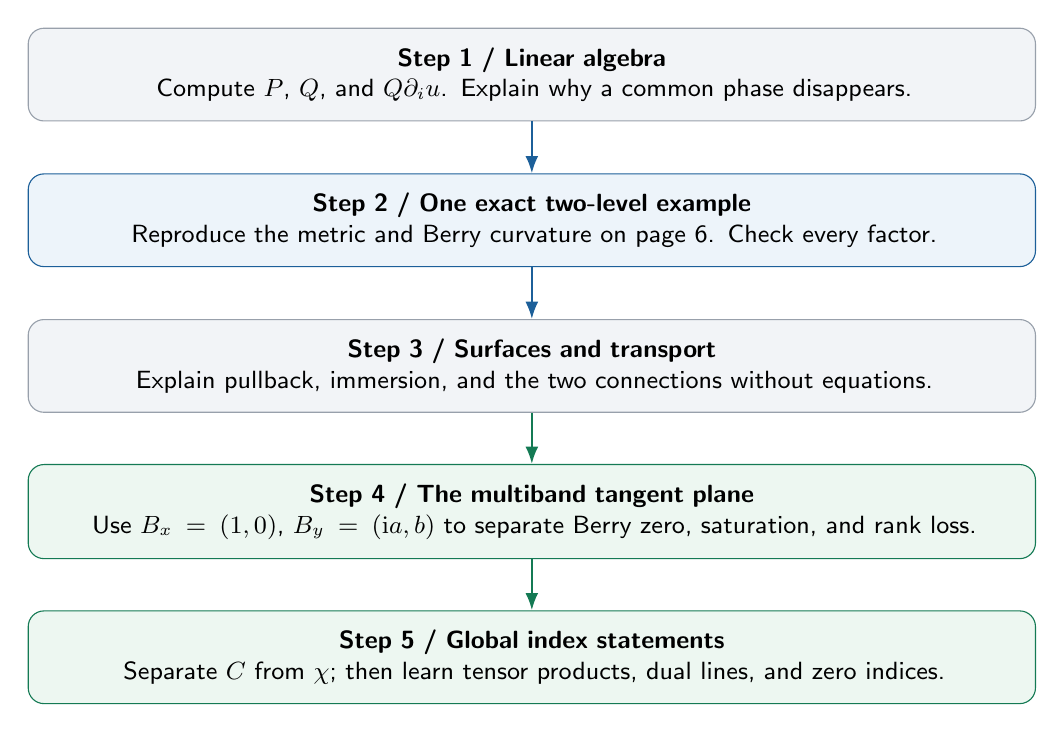
\begin{tikzpicture}
\node[basic,text width=12.3cm] (s1) at (0,0)
{\textbf{Step 1 / Linear algebra}\\
Compute $P$, $Q$, and $Q\partial_i u$. Explain why a common phase disappears.};
\node[known,text width=12.3cm] (s2) at (0,-1.85)
{\textbf{Step 2 / One exact two-level example}\\
Reproduce the metric and Berry curvature on page 6. Check every factor.};
\node[basic,text width=12.3cm] (s3) at (0,-3.7)
{\textbf{Step 3 / Surfaces and transport}\\
Explain pullback, immersion, and the two connections without equations.};
\node[proposed,text width=12.3cm] (s4) at (0,-5.55)
{\textbf{Step 4 / The multiband tangent plane}\\
Use $B_x=(1,0)$, $B_y=(\ii a,b)$ to separate Berry zero, saturation, and rank loss.};
\node[proposed,text width=12.3cm] (s5) at (0,-7.4)
{\textbf{Step 5 / Global index statements}\\
Separate $C$ from $\chi$; then learn tensor products, dual lines, and zero indices.};
\draw[flow] (s1)--(s2);
\draw[flow] (s2)--(s3);
\draw[eflow] (s3)--(s4);
\draw[eflow] (s4)--(s5);
\end{tikzpicture}
\end{center}
\smallhead{Read the supplied review selectively}
Start with Fig.\ 1 on p.\ 2, then IIA on pp.\ 4--6. Read IIIH on pp.\ 27--28
after the connection pictures. Read VD on pp.\ 50--51 for measurement scope.
The information-theory and many-body sections are valuable, but not
prerequisites for this three-paper story. \src{R}{contents and named sections}

\smallhead{Four short self-checks}
\begin{enumerate}
\item If $\ket{u(\mathbf k)}=e^{\ii\chi(\mathbf k)}\ket{u_0}$, can $\partial_i u$
be nonzero while the metric vanishes?
\item For $B_x=(1,0)$, $B_y=(0,1)$, find $g$, $\Omega$, and $\cos\theta_K$.
\item The two states of a two-level model have opposite Berry curvature.
Must they have opposite Gaussian curvature?
\item A three-band $C=-1$ example has five simple zeros with indices
$+,+,+,+,-$. Does this contradict the topological count?
\end{enumerate}
\begin{plainbox}
\textbf{Answers.}
(1) Yes: the derivative is pure gauge; $P$ is constant and $Q\partial_i u=0$.
(2) $g=I_2$, $\Omega=0$, $\cos\theta_K=0$.
(3) No: their metrics are identical, so their Gaussian curvatures agree.
(4) No: the signed sum is $3=-3C$, while the unsigned count is $5$.
\end{plainbox}

% PAGE 20: REFERENCES
\guidepage{19. Sources and how they are used}{Source codes appear beside relations and on the diagrams; all figures are newly drawn teaching schematics.}
\vspace{-3mm}
\begin{thebibliography}{H3}
\setlength{\itemsep}{4pt}
\small
\bibitem[R]{review}\hypertarget{ref:R}{}
A. Gao, N. Nagaosa, N. Ni, and S.-Y. Xu,
\emph{Quantum geometry phenomena in condensed matter systems},
Rev.\ Mod.\ Phys.\ \textbf{98}, 035005 (2026).
\href{https://doi.org/10.1103/f78t-ky69}{doi:10.1103/f78t-ky69}.
The user-supplied 67-page review. Printed p.\ 035005-$n$ is PDF page $n$.

\bibitem[H1]{h1}\hypertarget{ref:H1}{}
S.-M. Huang and D. Giataganas,
\emph{Exploring Grassmann manifolds in topological systems via quantum distance}.
\href{https://arxiv.org/html/2412.20046v2}{arXiv:2412.20046v2}.
Finite subspace comparison and projector-distance reconstruction.

\bibitem[H2]{h2}\hypertarget{ref:H2}{}
S.-M. Huang, \emph{Quantum-State Projectors on Grassmannian:
Geometry, Holonomy, and Topology}.
\href{https://arxiv.org/html/2608.06777v1}{arXiv:2608.06777v1}.
Projector tangents, QGT, geodesics, holonomy, and topology.

\bibitem[H3]{h3}\hypertarget{ref:H3}{}
S.-M. Huang, \emph{A Gauss-Bonnet Theorem for Quantum States:
Gauss Curvature and Topology in the Projective Hilbert Space}.
\href{https://arxiv.org/html/2510.15760v1}{arXiv:2510.15760v1}.
Two-band singular geometry; III--V are the core of the story here.

\bibitem[MO]{mo}\hypertarget{ref:MO}{}
B. Mera and T. Ozawa, \emph{K\"ahler geometry and Chern insulators:
Relations between topology and the quantum metric},
Phys.\ Rev.\ B \textbf{104}, 045104 (2021).
\href{https://arxiv.org/pdf/2103.11583}{arXiv:2103.11583}.
Pullback framework, two-band obstruction, and Appendix A's complex-tangent
saturation criterion.

\bibitem[AP]{ap}\hypertarget{ref:AP}{}
A. Avdoshkin and F. K. Popov, \emph{Extrinsic geometry of quantum states},
Phys.\ Rev.\ B \textbf{107}, 245136 (2023).
\href{https://arxiv.org/pdf/2205.15353}{arXiv:2205.15353}.
Appendix D supplies the ambient/tangent/normal decomposition and Gauss equation.

\bibitem[L]{lai}\hypertarget{ref:L}{}
H.-F. Lai, \emph{Characteristic classes of real manifolds immersed in complex
manifolds}, Trans.\ Amer.\ Math.\ Soc.\ \textbf{172}, 1--33 (1972).
\href{https://doi.org/10.1090/S0002-9947-1972-0314066-8}{doi:10.1090/S0002-9947-1972-0314066-8}.
Classical background to complex-point index formulas.

\bibitem[F]{forstneric}\hypertarget{ref:F}{}
F. Forstneri\v{c}, \emph{Stein domains in complex surfaces}.
\href{https://arxiv.org/pdf/math/0201097}{arXiv:math/0201097v3 (2003)}.
Equation (1.1) states the two combinations of complex-point indices for
oriented immersed surfaces.

\bibitem[E]{extension}\hypertarget{ref:E}{}
The multiband research notes supplied in this conversation, together with the
independent numerical verification summarized on 10 October 2026.
Unpublished working analysis; see the earlier
\texttt{kahler\_gauss\_audit\_2026-10-10.zip}.
Green indicates this proposed application, not a literature-priority judgment.
\end{thebibliography}
\vspace{-2mm}
\begin{cautionbox}
\textbf{Source discipline.} Standard facts and newly drawn pictures are not
new research claims. The three-paper narrative stays separate from [E].
We use H1's SVD and Hilbert--Schmidt formulas rather than its problematic
full-space trace expression (7), and do not universalize H3's specific
four-cusp counting formula. The optical response map uses the review's
(312)--(323); it does not infer a $K_{II}$ response from the shared word curvature.
\end{cautionbox}

% PAGE 21: TECHNICAL APPENDIX
\guidepage{Appendix A. The projector formulas behind the pictures}{Optional on a first reading. These identities make the proposed curvature calculation concrete.}
At a point choose a basis where $P=\operatorname{diag}(I_r,0)$.
Differentiating $P^2=P$ yields off-diagonal tangents:
\[
T_i=\partial_iP=
\begin{pmatrix}0&B_i^\dagger\\B_i&0\end{pmatrix},
\qquad
g_{ij}=\Ree\Tr(B_i^\dagger B_j).
\quad\src{H2}{IV.1--IV.2, (19)--(30)}
\]
The tangent projection onto the Grassmannian is
$\Pi_{\Gr}A=PAQ+QAP$.
Differentiating idempotency twice gives the normal part of the Grassmannian's
own embedding in flat Hermitian matrices:
\[
\mathcal N_{ij}=
\begin{pmatrix}
-(B_i^\dagger B_j+B_j^\dagger B_i)&0\\
0&B_iB_j^\dagger+B_jB_i^\dagger
\end{pmatrix}.
\quad\calc
\]
Insert this in the ordinary Gauss equation for that embedding, using
$\langle A,B\rangle=\frac12\Ree\Tr(A^\dagger B)$:
\[
\begin{split}
K_{\Gr}
&=\frac{\langle\mathcal N_{xx},\mathcal N_{yy}\rangle
-\|\mathcal N_{xy}\|^2}{\det g}\\
&=\frac{\|B_x^\dagger B_y-B_y^\dagger B_x\|_F^2
+\|B_xB_y^\dagger-B_yB_x^\dagger\|_F^2}{2\det g}.
\end{split}
\]
\src{AP}{Appendix D, Gauss identity}\quad\esrc{explicit block calculation}

For the Bloch surface \emph{inside} the Grassmannian, set
$A_{ij}=\Pi_{\Gr}(\partial_i\partial_jP)$ and subtract its surface-tangent part:
\[
II_{ij}=A_{ij}
-T_a\,g^{ab}\langle T_b,A_{ij}\rangle.
\]
Then use $K_G=K_{\Gr}+K_{II}$ from page 15.
This uses projectors and their derivatives, with no global eigenvector gauge.
\esrc{projector formula; requires an invertible pullback metric}

\smallhead{What was independently compared numerically}
The Gauss-equation result was compared with a Brioschi calculation made from
finite differences of the metric. The relative discrepancy was the maximum
absolute difference divided by the maximum absolute Brioschi curvature, on
the subset $\det g>10^{-3}\max_{\rm grid}\det g$.
\begin{center}
\begin{tabular}{@{}lccc@{}}
\toprule
Model & $120^2$ & $240^2$ & $480^2$\\
\midrule
Three bands, rank 1 & $2.88\,10^{-2}$ & $7.98\,10^{-3}$ & $1.86\,10^{-3}$\\
Four bands, rank 2 & $4.25\,10^{-2}$ & $1.11\,10^{-2}$ & $2.94\,10^{-3}$\\
\bottomrule
\end{tabular}
\end{center}
The decrease is consistent with second-order finite-difference convergence.
At $240^2$, the cutoff excludes about $0.9\%$ and $12.5\%$ of the respective
grids. The five confirmed complex points test the rank-one three-band index
sum; they do not certify that no additional canceling pairs exist.
\esrc{earlier verification archive}

\begin{plainbox}
\textbf{What you can now read in the original notation.}
$\partial P$ is a change of occupied subspace;
$g$ is its Gram matrix; $\Omega$ is a phase-curvature trace;
$II$ removes surface-tangent turning; the Gauss equation adds ambient
curvature and bending. Every one of these operations has a distinct physical
or geometric object.
\end{plainbox}
\end{document}
